%Documento elaborado através da modificação de Template_ Tese_ MAEG por RJF. 
%Com contribuições e modificações dos alunos do DEGGE e Phd student 
%Angelo Soares (arsoares@fc.ul.pt) com orientação de Carla M. Silva.
%11/11/2021
% Para escrever neste documento, expandam a secção Capitulos e escrevam no capitulo apropriado.
% Após a escrita, seleccionem "main.tex" e recompilem. Tudo o que escreverem nos capitulos irá 
% aparecer. 

% ------------------------------------------------------------------------------------------------------%
% ------------------------------------------ ALTERAR CAPA ----------------------------------------------%
% ------------------------------------------------------------------------------------------------------%
%A Neste main.tex as únicas alterações que precisam de fazer são referentes à Capa da
%dissertação. Sigam as indicações seguintes: Façam ctrl+F para procurar "includepdf" e leiam 
%as notas por baixo do \includepdf.

% ------------------------------------------------------------------------------------------------------%

%Outras Notas: 
%1. Ler o conteudo em "library.bib".
%2. O GOOGLE é vosso amigo, todas e quaisquer modificações necessárias, seja para introduzir um
%certo tipo de formatação, seja para colocar uma figura ou tabela com especificações particulares,
%usem o GOOGLE, existem N exemplos para todo o tipo de alteração em latex. Com quase copy+paste
%code.
% ------------------------------------------ IMPORTANTE -----------------------------------------------%
%3. Neste documento existem algumas colisoes de pacotes, nomeadamente o tocloft e o book report
%e a maneira %como o chapter foi elaborado. Exemplo: Se os alunos quiserem colocar o prefixo "1."
%antes da introdução, ou seja "1. Introdução". No Indice ficaria "1 1. Introdução".
%ALTERNATIVA: Escrevam a dissertação na totalidade. No fim, façam download do PDF (cliquem segundo
%Icone após o Recompile). Com esse ficheiro PDF, abram-no no PDF reader (adobe acrobat pro) e 
%editem acrescentando o número do capitulo para ficar igual ao que está no Indice "1. Introdução".
%É a forma mais simples de resolver.

%Se alguem por curiosidade encontrar outra solução usando o tocloft package, como por exemplo, 
%ocultar o número do capitulo no TOC sem usar \chapter* ou interferir com o hyperref enviem essa
%info para o email supramencionado, muito obrigado.
%Boa sorte


\documentclass[11pt,a4paper,twoside,openright]{book}
% ------------------------------------------------------------------------------------------------------%
% ------------------------------------------- PREAMBLE -------------------------------------------------%
% ------------------------------------------------------------------------------------------------------%
\usepackage{mathptmx} % Fonte mais próxima de Times New Roman
% Alterar margens do documento
\usepackage[margin=2.5cm]{geometry}
\renewcommand{\baselinestretch}{1.15}
\usepackage{setspace}
\usepackage{fancyhdr}
\usepackage{pgfplots}
\pagestyle{fancy}
\renewcommand{\chaptermark}[1]{\markboth{\MakeUppercase{\thechapter. #1 }}{}}
\renewcommand{\sectionmark}[1]{\markright{\thesection\ #1}}
\fancyhf{}
\fancyhead[RO]{\small{\rightmark}}
\fancyhead[LE]{\small{\leftmark}}
\setlength{\headheight}{12pt}
\addtolength{\topmargin}{-10.5pt}
\fancyfoot[C]{\thepage}
\renewcommand{\headrulewidth}{0pt}
\renewcommand{\footrulewidth}{0pt}
\addtolength{\headheight}{0.5pt}
\fancypagestyle{plain}{
  \fancyhead{}
  \renewcommand{\headrulewidth}{0pt}
}
\usepackage[utf8]{inputenc}
\usepackage{neuralnetwork}
\usepackage{datatool}
\usepackage{mathtools}
\usepackage[backend=biber, natbib=true, style=numeric-comp, sorting=none]{biblatex} %Numeric style
%\usepackage[backend=biber,style=authoryear,maxcitenames=1,autocite=inline,natbib=true]{biblatex}
%\addbibresource{library} %O ficheiro .bib que a bibliografia vai usar
%\bibliography{library}
%\addbibresource{library.bib} %O ficheiro .bib que a bibliografia vai usar
\bibliography{library}
\addbibresource{library.bib}


\usepackage{tikz}
    \usetikzlibrary{positioning, calc}
	\usetikzlibrary{fit}
	\usetikzlibrary{matrix, arrows}
 \usepgflibrary{shapes.misc} 
\tikzset{basic/.style={draw,fill=none,
                       text badly centered,minimum width=1.5em}}
\tikzset{input/.style={basic,circle,minimum width=1.75em}}
\tikzset{small_input/.style={basic,circle,minimum width=0.4em}}
\tikzset{weights/.style={basic,rectangle,minimum width=1em}}
\tikzset{neurons/.style={basic,rectangle,minimum width=1em, dashed}}
\tikzset{functions/.style={basic,circle, minimum width=2em}}
\newcommand{\addaxes}{\draw (0em,0.5em) -- (0em,-0.5em)
                            (-0.5em,0em) -- (0.5em,0em);}
\newcommand{\relu}{\draw[line width=0.75pt] (-0.5em,0) -- (0,0)
                                (0,0) -- (0.375em,0.375em);}
\newcommand{\stepfunc}{\draw[line width=0.75pt] (0.325em,0.325em) -- (0,0.325em) 
                                    -- (0,-0.325em) -- (-0.325em,-0.325em);}
%\bibliographystyle XXX
%\usepackage[numbers]{natbib}1
\usepackage{nicematrix}
% Package que permite incluir imagens
\usepackage{graphicx}
% Comentar para não incluir a lista de figuras e tabelas no índice
\usepackage[nottoc]{tocbibind}

% Para citar referências
%\usepackage{natbib}
%\setcitestyle{numbers}
%\bibliographystyle{humannat}
%\setcitestyle{authoryear}

%Indentar primeiro parágrafo
\usepackage{indentfirst}

% Incluir até à subsecção no índice
\setcounter{tocdepth}{3}
\setcounter{secnumdepth}{3}

% Permite remover os espaços entre itens
\usepackage{enumitem}

% Caption para imagens
\usepackage[font=footnotesize]{caption}

% Referenciar anexos
\usepackage[toc,page]{appendix}

%Adicionar pdfs
\usepackage{pdfpages}

%Alterar nome de capitulo para a referencia
\usepackage{fmtcount}
\usepackage{url}

%Para expressões Matemáticas
\usepackage{amsmath}
\usepackage{bm}

%Bibliotecas
\usepackage{biblatex}
%\usepackage[portugues]{babel} %Can be switched to english
%\usepackage{csvsimple}
\usepackage{csvsimple-l3}
\usepackage{float}
\raggedbottom
\usepackage{subcaption}
\usepackage{eurosym}
\usepackage{booktabs}
\usepackage{ragged2e}
\usepackage[T1]{fontenc}
\usepackage{csquotes}
\usepackage{tabularx}
%\usepackage[scaled]{helvet}
%\renewcommand*\familydefault{\sfdefault}

%Comando que cria abreviaturas usado no Nomenclatura
\newcommand{\abbreviations}[1]{%
\vspace{12pt}\noindent{\selectfont\textbf{Abreviaturas}\par\vspace{6pt}\noindent {\fontsize{9}{9}\selectfont #1}\par}}
%Criar Siglas
\newcommand{\siglas}[1]{%
\vspace{12pt}\noindent{\selectfont\textbf{Siglas e acrónimos}\par\vspace{6pt}\noindent {\fontsize{9}{9}\selectfont #1}\par}}
%Cria simbologia
\newcommand{\simbolos}[1]{%
\vspace{12pt}\noindent{\selectfont\textbf{Simbologia}\par\vspace{6pt}\noindent {\fontsize{9}{9}\selectfont #1}\par}}

\makeatletter
\def\cleardoublepage{\clearpage\if@twoside \ifodd\c@page\else
    \hbox{}
    \thispagestyle{plain}
    \newpage
    \if@twocolumn\hbox{}\newpage\fi\fi\fi}
\makeatother \clearpage{\pagestyle{plain}\cleardoublepage}

\providecommand{\keywords}[1]{\textbf{Keywords:} #1}
\providecommand{\keywordsP}[1]{\textbf{Palavras chave:} #1}

%Remover Chapter N on the header
\usepackage{titlesec}
\usepackage{lipsum}
\titleformat{\chapter}[display]
   {\normalfont\huge\bfseries}{\chaptertitlename\ \thechapter}{20pt}{\Huge}   
\titlespacing*{\chapter}{0pt}{-20pt}{40pt}
\titleformat{\chapter}[display]{\normalfont\bfseries}{}{0pt}{\huge}

%\numberwithin{section}{chapter}
\usepackage{multirow}
\usepackage{chngcntr}  
\usepackage{tocloft}
\usepackage[hidelinks]{hyperref}
\hypersetup{
    colorlinks=true,
    linkcolor=black,  % color of internal links
    filecolor=black,  % color of links to local 
      urlcolor=blue,
}
%\counterwithout{figure}{chapter}
%\counterwithout{table}{chapter}

\renewcommand{\cftfigpresnum}{\textbf{Figura\ }}
\renewcommand{\cfttabpresnum}{\textbf{Tabela\ }}

\newlength{\mylenf}
\settowidth{\mylenf}{\cftfigpresnum}
\setlength{\cftfignumwidth}{\dimexpr\mylenf+1.5em}
\setlength{\cfttabnumwidth}{\dimexpr\mylenf+1.5em}

\sloppy

\makeatletter
\newcommand\listoftablesandfigures{%
    \chapter*{List of Tables and Figures}%
    \phantomsection
\@starttoc{lof}%
\bigskip
\@starttoc{lot}}
\makeatother

\PassOptionsToPackage{hyphens}{url}\usepackage{hyperref}

% ------------------------------------------------------------------------------------------------------%
% ------------------------------------------- END - PREAMBLE -------------------------------------------%
% ------------------------------------------------------------------------------------------------------%

\begin{document}


% Capa
\newpage
\thispagestyle{empty}

%\setmainfont[Path = fonts/]{arial_narrow.ttf} 

\centering{\fontsize{12.2}{14.4}\selectfont UNIVERSIDADE DE LISBOA}\\
\centering{\fontsize{12.2}{14.4}\selectfont FACULDADE DE CIÊNCIAS}\\
\centering{\fontsize{12.2}{14.4}\selectfont DEPARTAMENTO DE ENGENHARIA GEOGRÁFICA,GEOFÍSICA E ENERGIA}

\vspace{1.3cm}

\begin{figure}[h]
 \centering
 \includegraphics[width = 6.99cm,height = 3.3cm]{Imagens/logo_fcul.png}
\end{figure}

\vspace{3.45cm}

%\setmainfont[Path = fonts/]{arial_narrow_bold.ttf}

\centering{\fontsize{17}{20.4}\selectfont \textbf{Participação da geração renovável no mercado de reservas de um sistema eléctrico}}

%\setmainfont[Path = fonts/]{arial_narrow.ttf}

\vspace{4cm}

\centering{\fontsize{14}{16.8}\selectfont João Pedro Passagem dos Santos}

\vspace{1.3cm}

%\setmainfont[Path = fonts/]{arial_narrow_bold.ttf}

\centering{\fontsize{13}{15.6}\selectfont \textbf{Mestrado em Engenharia da Energia e Ambiente}}\\

%\setmainfont[Path = fonts/]{arial_narrow.ttf}

%\centering{\fontsize{13}{15.6}\selectfont Especialização em Bioinformática}

\vspace{0.5cm}


\vspace{0.5cm}

\centering{\fontsize{13}{15.6}\selectfont Dissertação orientada por:}\\
\centering{\fontsize{13}{15.6}\selectfont Doutor Hugo Algarvio}\\
\centering{\fontsize{13}{15.6}\selectfont Professora Doutora Ana Estanqueiro}\\

\vspace{2.9cm}

\centering{\fontsize{14}{16.8}\selectfont 2024}
\label{Capa}



\let\cleardoublepage\clearpage


\clearpage \thispagestyle{empty}\mbox{}\clearpage

\frontmatter
% RESUMO
\newpage
\thispagestyle{plain}
\chapter{Resumo}
\justifying

A crescente penetração de fontes de energia renováveis variáveis no tempo, \gls{vRES}, no sistema eléctrico, como a solar e a eólica, está a transformar significativamente os mercados de eletricidade, devido à sua natureza intermitente e imprevisível. Esta imprevisibilidade torna as previsões de produção e consumo de energia mais desafiantes, especialmente porque os mercados de eletricidade fecham entre 1 e 37 horas antes da entrega real da energia, o que pode resultar em discrepâncias entre a energia contratada e a energia realmente produzida ou consumida. Manter o equilíbrio entre a oferta e a procura em tempo real é vital para a segurança e estabilidade da rede, função que recai principalmente sobre os operadores de redes de transporte (\gls{TSO}).\par
Os \gls{TSO} utilizam mercados de reserva de energia, onde adquirem de forma simétrica potência secundária ascendente e descendente, com base em previsões de procura para as horas subsequentes. No entanto, essa abordagem simétrica pode ser ineficaz diante das flutuações das energias renováveis, levando à necessidade de ajustes mais dinâmicos e precisos.\par
Neste contexto, o presente trabalho propõe primeiramente um estudo do parâmetro variável por hora da fórmula do \gls{TSO} português para a previsão de reserva necessária ($\rho$), onde usando os dados históricos horários no período 2010 a 2019, é calculado o $\rho$ horário que resulte num menor erro médio na previsão, onde são obtidos resultados com erro inferior a 5\%.\par
Este trabalho propõe de seguida um modelo baseado em técnicas de \textit{machine learning} para calcular dinamicamente as reservas de potência secundária, tanto ascendente como descendente, integrando despachos programados para o dia seguinte, previsões de produção de \gls{vRES}, a procura prevista e outras características operacionais.\par
Utilizando dados operacionais abertos do \gls{TSO} espanhol, o modelo foi treinado com dados no período de 2014 a 2023,  e validado com dados de referência de 2019 a 2022. A metodologia proposta demonstra uma melhoria significativa na utilização das reservas de potência secundária, com um aumento de aproximadamente 43\% na eficiência das reservas ascendentes e cerca de 36\% nas reservas descendentes. Este avanço contribui para uma gestão mais eficiente e equilibrada do sistema elétrico, especialmente em cenários com elevada penetração de \gls{vRES}.\par




\vspace{0.5cm} %adiciona um espaço de 0.5cm entre o texto e as palavras chave.

\keywordsP{sistemas de reserva, mercados de energia, redes neuronais, previsões}
%reparem que # necessita de um \ para que o latex o interprete correctamente como um caracter especial. Isto também acontece com % por exemplo.
\label{resumo}

%Abstract
\newpage
\thispagestyle{plain}
\chapter{Abstract}
Abstract should have the relevant information of the developed work. One sentence with the framework of the research. One sentence with the goal and method. One sentence with the main conclusions.

\vspace{0.5cm} %adds a 0.5cm space between the text and the keywords.

\keywords{up to six different from the title and helpful to find related subjects (like \# in social media)} 
%notice that # requires a \ so that latex correctly interprets it as a special character. This also happens with % for example.
\label{abstract}

% AGRADECIMENTOS
\newpage
\thispagestyle{plain}
\chapter{Agradecimentos}
Opcional, embora no caso de dissertações que decorram no âmbito de projetos financiados, por exemplo, pela FCT ou programas europeus devem ser mencionados aqui a referência e nome do projeto, e mais alguma informação conforme as regras de publicitação do projeto em questão.

\vspace{10mm} %ele aceita diversos tipos units, neste caso 10mm, 0.1cm.

\flushleft{Nome do Autor}
\label{agradecimentos}

%Nomenclatura
\newpage
\thispagestyle{plain}
\chapter{Nomenclatura}
% Lista de siglas, acrónimos, abreviaturas e simbologia apresentadas por ordem alfabética.

% %Utilizar sempre \\ para forçar a mudança de linha.
% %Utilizar o & para forçar a mudança de "coluna", como numa tabela
% \abbreviations{\noindent 
% \begin{tabular}{@{}ll}
% (A/F) & Relação mássica ar/combustível\\
% pme	& Pressão média efectiva\\
% vol & Volume\\
% \end{tabular}
% }
\vspace{12pt}
\printglossary[type=\acronymtype, title={Siglas e acrónimos}, style=customstyle]


\simbolos{\noindent 
\begin{tabular}{@{}ll}
Hz & Hertz\\
MW & Megawatts\\
MWh & Megawatt-hora\\
\end{tabular}
}
%The use of \( \) avoids obscure compiling errors in latex when using certain mathematical notation symbols in a non-mathematical environment (text).
%https://tex.stackexchange.com/questions/510/are-and-preferable-to-dollar-signs-for-math-mode

%Nota: List of greek letters and others https://pt.overleaf.com/learn/latex/List_of_Greek_letters_and_math_symbols
\label{ch:nomenclatura}

% ÍNDICE
% ÍNDICE (Não é preciso fazer nada, faz update automaticamente)
\clearpage
\thispagestyle{plain}
\renewcommand{\contentsname}{Índice}
\tableofcontents
\clearpage
\thispagestyle{plain}
\listoffigures
\clearpage
\thispagestyle{plain}
\listoftables
\clearpage \thispagestyle{plain}\mbox{}\clearpage

\mainmatter
\setlength{\parindent}{15pt} %Comentar retira a indentação inicial nos chapters
\pagenumbering{arabic} %numeros em numeração árabe

% INTRODUÇÃO
\newpage
\thispagestyle{plain}
\chapter{Introdução}

\section{Enquadramento\label{se:enquadramento}}
Esta dissertação enquadra-se no âmbito do projeto \href{https://traderes.eu/}{TradeRES}, que visa o estudo de um sistema de mercado eléctrico capaz de atender às necessidades da sociedade num sistema quase totalmente renovável, tendo as características para se integrar nos \href{https://ods.pt/ods/}{ \gls{ODS}} \ref{fig:ODS}.\par
O estudo da acessibilidade das energias renováveis ao mercado vigente integra-se nos \gls{ODS} n$^{\circ}$7, “Energia Renováveis e Acessíveis”, indo directamente de encontro a um dos pontos deste objectivo: 7.2.1 “Peso das energias renováveis no consumo total final de energia”. Por meio deste objectivo, a participação das renováveis no mercado faz também cumprir, embora indiretamente, o objectivo n$^{\circ}$8 “Trabalho Digno e Crescimento Económico”, através do ponto 8.4, onde, neste último, é dada primazia à eficiência dos recursos globais no consumo e na produção. Esta contribuição indireta ocorre através da diminuição do uso de energias não limpas, justificadas por um maior uso das renováveis, melhorando a gestão de recursos, e baixando o consumo de recursos naturais não renováveis.\par
Por último, no âmbito do presente estudo, podemos igualmente incluir o objectivo n$^{\circ}$13, “Acção Climática”, no qual, referimos, não só a diminuição de consumo de recursos finitos, mas ainda, a melhor gestão de recursos renováveis, promovendo o planeamento e estratégias de combate a emissões de gases de efeito estufa.\par

\begin{figure}[h]
    \centering
    \includegraphics{Imagens/DesenvolvimentoSustentavel.jpg}
    \caption{Objectivos de Desenvolvimento Sustentável da ONU}
    \label{fig:ODS}
\end{figure}

\section{Objetivos e Perguntas de Pesquisa\label{se:objetivos}}

Foram aprovadas a nível europeu (2020)\cite{52020DC0299} sugestões de alterações aos serviços de sistema, que serão seguidas pelos Estados-Membros. Nesta dissertação, será realizada a aplicação dessas sugestões, identificando as melhorias em relação ao \textit{design} actual e avaliando se as novas sugestões serão suficientes para garantir a operação de um sistema elétrico \textasciitilde100\% renovável, potencialmente identificando ações adicionais para garantir a robustez e segurança do sistema elétrico sem o uso de combustíveis fósseis.\par
A penetração das \gls{vRES} no sistema de energia eléctrica trouxe maior incerteza na previsão em mercados de energia, pois estas estão mais sujeitos a elementos não controláveis como a velocidade do vento ou a radiação solar incidente.\par
As seguintes perguntas servirão de guia nesta pesquisa:\par

\begin{enumerate}[label=\alph*)]
  \item Podemos reduzir a incerteza na produção criada pela participação das \gls{vRES} nos sistemas de energia? 
  \item A alocação dinâmica pode ter um efeito positivo no mercado de reservas?
  \item É possível prever a necessidade de reserva necessária baixando a alocação desperdiçada?
\end{enumerate}

Para responder às perguntas \textit{supra} referidas, utilizaremos dados de previsão de geração de energia renovável para estimar a energia necessária para alocação secundária. Actualmente, os valores de previsão desse mercado estão distantes do consumo real, o que resulta em alocações no dia anterior que não estão em conformidade com as necessidades reais.\par
O objetivo deste trabalho é criar métodos de previsão para o dia seguinte, da necessidade de alocação de banda de reserva secundária, de modo a alocar banda suficiente e, simultaneamente, baixar a alocação em excesso, usando dados históricos das mesmas.\par
Iremos explorar a optimização da fórmula de alocação de banda de reserva da REN, testando novos valores para o parâmetro horário da mesma.\par
Utilizando técnicas de \textit{machine learning} vamos criar um modelo para a previsão de alocação necessária do dia seguinte.\par
Previsões mais exactas tornam possível uma melhor gestão das alocações, resultando num menor gasto de recursos energéticos e financeiros.\par

\section{Organização do Documento \label{se:organização}}

Este documento está dividido em capítulos. Sendo que os primeiros apresentam uma introdução às ideias e temas no 1, o estado de arte dos temas na literatura publicada, seguido de uma contextualização do tema do trabalho proposto no capítulo 2. Dentro da contextualização é de forma geral apresentado os mercados de energia, os sistemas de reserva, e os métodos de previsão para os mesmos, dentro destes o uso de fórmulas e o uso de \textit{machine learning}, formulando aqui a motivação e caminho de estudo.\par
No capítulo 3 apresentamos no sub-capítulo Ferramentas as bibliotecas criadas em \textit{python} para o presente estudo.
Segue o sub-capítulo Métodos onde abordamos os diferentes estudos presentes, como serão dirigidos e condições a alcançar. Dividindo o trabalho em estudos distintos para o tipo de previsões apresentadas no capítulo 2.
Métricas e Dados intitula o capítulo 4 que começa numa dissecção das métricas aplicadas ao longo das experiências e como estas influenciam a mesma, terminando num estudo geral dos dados utilizados, seus tratamentos e elações iniciais de análise. Apresentado também o que é usado como treino e como validação para as experiências.
No capítulo 5 são apresentados os resultados da experiência completa, incluindo as métricas apresentadas, apresentado gráficos de séries temporais das previsões conseguidas. Dando realce aos melhores modelos e optimizações conseguidos.
Termina com um breve capítulo conclusivo dando um pouco mais de contexto aos resultados, apresentando possíveis caminhos futuros de melhoria dos mesmos e discutindo o impacto de \textit{machine learning} no futuro das energias renováveis e consequentemente nos mercados de reserva.

% Os dois capítulos seguintes apresentam os dois diferentes estudos. No \hyperref[ch:estudo_1]{capítulo 4} é definido e apresentado o resultado do estudo da estimativa do parâmetro $\rho$ da fórmula de estimativa da \gls{REN}.\par
% No \hyperref[ch:estudo_2]{capítulo 5} explora-se o segundo estudo, o dimensionamento dinâmico da alocação necessária. São apresentados os dados utilizados com um estudo preliminar sobre os mesmos, e o tratamento necessário para usar nos modelos.\par
% No \hyperref[ch:ferramentas]{capítulo 6} as ferramentas de programação criadas para realizar a mesma.\par
% Os 3 capítulos seguintes são os descritivos da experiência em si. \hyperref[ch:metricas]{Capítulo 7} são as métricas usadas e criadas para a validação da experiência, \hyperref[ch:metodos]{capítulo 8} é a estrutura e parametrização da mesma, e \hyperref[ch:resultados_discussao]{capítulo 9} apresenta os resultados.\par
% Termina com um \hyperref[ch:conclusao]{capítulo conclusivo} onde são avaliadas as experiências como um todo, e o seu impacto no âmbito dos mercados de reserva.\par
\label{ch:intro}

% Revisão bibliográfica
\newpage
\thispagestyle{plain}
\chapter{Revisão bibliográfica}

A análise de séries temporais é um tema recorrente em pesquisa. Especialmente para previsões.\\
Desde as previsões para mercados de acções\cite{Bhandari2022}, fenomenos meteorologicos\cite{Wang2019}, e especialmente mercados energéticos, onde se quer ter em consideração o impacto das gerações mais voláteis. \\
As energias renováveis, devido à sua natureza, são as produçoes mais voláteis, logo alvo de estudo ideal para estas tecnologias\cite{Lu2015}
, energia eolica\cite{Sun2022}, energia solar\cite{Rajasundrapandiyanleebanon2023}, aplicabilidade dos vários sistemas\cite{Ahmad2020}, procura\cite{Antonopoulos2020}.
Sendo que cada problema já apresenta arquiteturas e soluções diferentes, como a geração de energia fotovoltaica em casas pode ser melhor prevista com LSTM\cite{Costa2022} mas tambem com uso de SVM\cite{Meenal2018}
As várias faces destas tecnologias estão optimamente apresentadas em\cite{Benti2023}



Para o estudo de previsões de séries temporais chega a ser o caso se pesquisar primeiramente com \textit{deep learning}, antes de procurar outras soluções.\\
Em \cite{Elsayed} é visto o impacto dessa decisão, e se realmente compensa emergir em \text{machine learning}. O trabalho conclui que modelos simples, com alguma engenharia de atributos inteligente, consegue competir, ou mesmo passar as qualidades de redes neuronais profundas. \\
Esta conclusão mostra também que por vezes a procura por modelos mais complexos não compensa, e que cada problema/dataset deve ter a sua própria investigação e conclusão, consoante a quantidade/qualidade de recursos disponiveis. \\

Os sistema de reserva de frequência do mercado espanhol já foram alvo de análise predictivas com modelos de redes neuronais profundas \cite{miota2023}.\\
Neste trabalho procurou-se prever o preço da banda de reserva secundaria, sendo que os melhores modelos atigiram metricas de MASE de cerca de 64\%, o que não foi considerado um bom resultado. \\
Para o trabalho presente, isto mostra que a resolução linear destes dados pode ser dificil. O trabalho utilizou 32 variaveis abertas pela TSO espanhola, e tambem conclui que o aumento de numero de variveis não melhorou os modelos. Para este trabalho o impacto deste conhecimento é pouco, visto estudarmos com um conjunto fixo de variaveis, e sendo que queremos perceber se conseguimos prever com esse conjunto.\\
Embora estes dados tragam um estudo parecido, usando dados da mesma fonte, o objectivo é ligeiremente diferente.








\label{ch:revisao}

% Contextos
\newpage
\thispagestyle{plain}
\chapter{Contextos\label{ch:contextos}}

\section{Mercado de Serviços de Sistema \label{se:servicos_sistema}}
%\cite{Lopes2021}
%\cite{Watson1984}
%\citep{Schweppe1988}

% O mercado de serviço de sistema é parte integrante dos mercados de energia e mantêm responsabilidade sobre a segurança do mesmo.\cite{dgegmss}.
% Serve para garantir o equilíbrio entre a energia produzido e a consumida. Esta qualidade e segurança é controlada através da frequência e da potência activa, controlo de tensão e potência reactiva, arranque automático e outras técnicas de sistemas \cite{Rassid2017} \cite{Carneiro2016}. \\
% Neste caso de estudo estamos interessados nos serviços de controlo de frequência. A nível europeu estes serviços são impostos pela \gls{ENTSO-E}, e a operação dos mesmos é da responsabilidade dos \gls{TSO} nacionais.\\
% Para manter o controlo de frequência o gestor de sistema deverá manter reservas para responder às diferenças entre a energia consumida e produzida na rede, que deve ser mantida em equilíbrio. Quando o serviço de sistema precisa de actuar para manter a frequência no seu valor nominal, 50Hz na Europa, isto é feito alterando a potência activa dos geradores.  \\
% Quando é necessário um aumento na potência chama-se a isto Banda de Reserva/Regulação a Subir, e quando é necessária uma diminuição chama-se à mesma a Descer.
% Para isto, no mercado ibérico, a tarefa é dividida em três reservas, primária, secundária e terciária. Esta divisão assenta no tempo de resposta que os sistemas precisam de ter, e na capacidade de actuação (MWh/Hz). \\

% A reserva primária é a primeira a ser activada em resposta a distúrbios na rede, como desvios de frequência, e deve agir em questão de segundos para estabilizar o sistema. A reserva secundária, que funciona como um sistema de segurança para a reserva primária, é regulada pelo mercado de banda das reservas secundárias, e sua alocação ocorre no dia anterior à sua necessidade. A reserva terciária é usada para complementar as reservas anteriores e para lidar com desvios de potência activa de longa duração.
% O valor alocado de reserva secundária tem um custo para as operadoras, como tal a previsão do mesmo é importante para a gestão destes sistemas de segurança. Estas previsões são feitas através de estatísticas dos sistemas, e tendo em conta as áreas de balanço que os mesmos têm.\\
% Assim como no mercado de energia de balanço, onde a participação de \gls{vRES} é cada vez mais incentivada, também nos serviços de reserva há uma crescente necessidade de adaptar esses mercados para acomodar a variabilidade e a imprevisibilidade inerente das \gls{vRES}, como a energia eólica e solar. A falta de harmonização nos mercados de balanço, particularmente na forma como os preços de desequilíbrios são determinados, apresenta um desafio significativo. Embora a participação de produtores de energia renovável nesses mercados seja tecnicamente viável, existem restrições que visam garantir a segurança e a estabilidade da rede, além de questões económicas que precisam ser abordadas para tornar esses mercados mais atrativos para todos os participantes.\\

% Uma previsão precisa das necessidades de reservas secundárias é crucial, pois impacta diretamente os custos e recursos das operadoras.
% Estas previsões são feitas usando fórmulas. Que por si só não prevêem a variabilidade dos sistemas de produção de energia renovável. Esta variabilidade sendo dificilmente previsível, tem sido alvo de estudo com modelos de \textit{machine learning}.\\
% Com o aumento de dados históricos destes mercados começa a ser possível estudar os mesmos para criar métodos empíricos para estas previsões.\\
% Com bons resultados apresentados em estudo de energias renováveis, a aplicação dos mesmos métodos para as reservas de sistema parece um passo natural. \\


\subsection{Introdução ao Mercado de Serviços de Sistema \label{se:intro_servicos_sistema}}

O mercado de serviços de sistema é uma componente fundamental dos mercados de energia, desempenhando um papel crucial na manutenção da segurança e estabilidade das redes elétricas \cite{dgegmss}. Esses serviços são essenciais para garantir que a produção e o consumo de energia permaneçam em equilíbrio, um requisito vital para o funcionamento seguro e eficiente de qualquer sistema eléctrico. A principal função dos serviços de sistema é assegurar a qualidade da energia fornecida, monitorizando parâmetros críticos como a frequência, a potência activa e reactiva, controlando a tensão na rede, arranque automático e outras técnicas de sistemas. Esse controlo é realizado através da coordenação entre os geradores e os consumidores, com o objetivo de responder rapidamente a variações na oferta e na procura de energia \cite{Rassid2017} \cite{Carneiro2016}.\\
No contexto europeu, a regulação desses serviços é coordenada pela \gls{ENTSO-E}, que estabelece os requisitos e normas para a operação dos sistemas de energia, e a operação dos mesmos é da responsabilidade dos \gls{TSO} nacionais. Essas reservas são activadas conforme necessário para manter a frequência da rede no seu valor nominal de 50Hz, ajustando a potência activa dos geradores em resposta a variações imprevistas na demanda ou na oferta de energia.\\
As reservas de frequência são divididas em três categorias principais: primária, \gls{FCR}, secundária, \gls{aFRR} e terciária, \gls{mFRR}. Cada uma com funções específicas e tempos de resposta distintos. A reserva primária é activada automaticamente e de forma quase instantânea, dentro de segundos após um distúrbio na rede, para estabilizar rapidamente a frequência. A reserva secundária entra em ação logo em seguida, substituindo gradualmente a reserva primária e ajustando a frequência de volta ao seu valor programado. Finalmente, a reserva terciária é utilizada para corrigir desvios de longo prazo e libertar as outras reservas para possíveis eventos futuros, completando o ciclo de controlo da frequência e assegurando que o sistema retorne a um estado de equilíbrio estável.\\
A harmonização dos mercados europeus de eletricidade, especialmente nos mercados diários, intradiários e de balanço, é uma realidade em desenvolvimento que busca reduzir custos e melhorar as condições de participação para todos os envolvidos \cite{Algarvio2019}. No entanto, a integração das \gls{vRES}, como a eólica e a solar, apresenta desafios adicionais devido à sua natureza intermitente e dependente de condições climáticas. Embora tecnicamente viável, devido a este paradigma de imprevisibilidade e ao facto de serem fontes não despacháveis, a participação dessas fontes nos mercados de balanço enfrenta restrições significactivas para garantir a segurança e a estabilidade da rede.\\
A atual infraestrutura dos mercados de serviços de sistema precisa, portanto, ser adaptada para acomodar essas novas fontes de energia. Uma parte essencial dessa adaptação é o desenvolvimento de métodos mais robustos para prever a necessidade de reservas, que levem em consideração a variabilidade das \gls{vRES}. Actualmente, as previsões são baseadas principalmente em fórmulas criadas pelas operadoras, mas esta abordagem muitas vezes falha em capturar a complexidade e a incerteza associadas à produção renovável. Assim, há uma crescente exploração de técnicas avançadas, como o uso de modelos de \textit{machine learning}, para melhorar a precisão das previsões e otimizar a gestão das reservas.
Além disso, a evolução para um mercado pan-europeu harmonizado de serviços de sistema envolve não apenas a uniformização de regras e requisitos técnicos, mas também a criação de incentivos económicos que tornem a participação atraente para todos os tipos de produtores de energia, incluindo os renováveis. Isso é particularmente importante, uma vez que os mercados de balanço são fundamentais para garantir que as redes elétricas possam operar de forma estável e segura, mesmo com altas penetrações de \gls{vRES}. Ao permitir que essas fontes renováveis participem de forma mais activa e competitiva nos mercados de balanço, espera-se não apenas reduzir os custos de operação dos sistemas eléctricos, mas também aumentar a viabilidade económica das \gls{vRES}.\\
Com a crescente dependência de fontes de energia renovável e a necessidade de sistemas eléctricos mais resilientes e flexíveis, o papel dos serviços de sistema continuará a expandir-se e a evoluir, exigindo inovações tanto na gestão técnica quanto na regulação econômica dos mercados de energia.\\


\subsection{Estrutura e Funcionamento das Reservas de Frequência \label{se:reservas_freq}}


A reserva primária, \gls{FCR}, é o primeiro nível de resposta e é acionada automaticamente em questão de segundos após a detecção de um desvio de frequência, que pode ocorrer devido a falhas na produção ou variações repentinas na procura. Esta reserva é activada até 15 segundos após o distúrbio e permanece activa por cerca de 30 segundos, ou até que a reserva secundária possa assumir o controlo. A \gls{FCR} é geralmente suportada por geradores que possuem capacidade técnica para resposta rápida, como hidroelétricas e algumas unidades térmicas. Este serviço é obrigatório para todos os geradores conectados à rede que possuem a capacidade técnica necessária, e não é remunerado em muitos mercados europeus, incluindo o mercado ibérico.\\
A reserva secundária \gls{aFRR} entra em ação logo após a activação da reserva primária, com o objetivo de restaurar a frequência da rede ao seu valor programado de 50 Hz e libertar a \gls{FCR} para responder a possíveis distúrbios subsequentes. A \gls{aFRR} é activada automaticamente até 30 segundos após o desvio inicial e pode levar até 15 minutos para corrigir completamente o desequilíbrio. Este tipo de reserva é contratado em mercados específicos de banda de reserva, nos quais os geradores submetem ofertas para fornecer a capacidade necessária.\\
A reserva terciária \gls{mFRR} é o último nível de resposta e é utilizada principalmente para corrigir desequilíbrios de longo prazo e libertar a \gls{aFRR} para outros usos. Ao contrário das reservas primária e secundária, a \gls{mFRR} é activada manualmente pelos \gls{TSO} e pode levar até 15 minutos a estar completamente activa. Esta reserva é frequentemente utilizada para ajustar a geração ou o consumo de energia de acordo com desvios significativos e prolongados, que não podem ser compensados de forma eficaz pelas reservas de resposta mais rápida. A \gls{mFRR} é geralmente suportada por geradores que podem oferecer flexibilidade em suas operações, como algumas centrais térmicas e hidroelétricas de grande porte.\\

\subsection{Previsão de Necessidades de Reservas \label{se:pred_impact_vres}}

A previsão das necessidades de reservas de frequência é uma componente essencial na gestão eficiente dos sistemas eléctricos, especialmente num cenário de crescente penetração das \gls{vRES}.\\
O uso de técnicas de \textit{machine learning} tem sido explorado como uma solução promissora para melhorar essas previsões. Estes modelos podem analisar grandes volumes de dados, identificar padrões complexos e ajustar previsões em tempo real, levando em consideração factores como mudanças nas condições meteorológicas e padrões de consumo de energia. Ao incorporar a variabilidade das \gls{vRES} nos modelos de previsão, é possível reduzir a incerteza e melhorar a alocação das reservas de frequência, resultando numa operação mais eficiente do sistema eléctrico.\\
Outro factor crítico na previsão das necessidades de reservas de frequência é a coordenação entre diferentes mercados e operadores de sistemas. A harmonização dos mercados europeus de balanço, incluindo a padronização das regras de oferta, leilão e remuneração, pode facilitar a integração das \gls{vRES} e melhorar a eficiência geral do sistema. Com regras claras e uniformes, os produtores de energia renovável têm maior incentivo para participar activamente dos mercados de reservas, fornecendo capacidade adicional para apoiar a estabilidade da rede. Isso é particularmente relevante em mercados onde as \gls{vRES} ainda enfrentam barreiras significactivas para a participação, como regras complexas de licitação ou altos requisitos de capacidade mínima para participação.\\
Apesar dos avanços na previsão de necessidades de reservas, ainda existem desafios consideráveis. A precisão das previsões pode ser limitada pela qualidade dos dados disponíveis, bem como pela capacidade dos modelos de capturar todas as variáveis relevantes que afetam a operação da rede. Além disso, a crescente interconexão dos sistemas eléctricos e o aumento da troca de energia entre países exigem uma abordagem coordenada e colaboractiva para a previsão de reservas, considerando tanto as condições locais quanto regionais.\\
O desenvolvimento contínuo de técnicas avançadas de previsão e a integração de soluções baseadas em dados serão fundamentais para enfrentar esses desafios. À medida que mais dados históricos se tornam disponíveis e os modelos de previsão evoluem, espera-se que a gestão das reservas de frequência se torne cada vez mais eficiente, contribuindo para um sistema eléctrico mais resiliente e capaz de integrar altos níveis de energias renováveis. Isso não apenas reduzirá os custos operacionais, mas também contribuirá para a segurança energética e para a transição para um sistema energético mais sustentável.\\


%\section{\gls{MIBEL} \label{se:mibel}}
%\cite{Bessa2012}
%\cite{Fernandes2016}
%\citep{Agostini2021}


\thispagestyle{plain}
\section{Arquitecturas de Modelos\label{se:arquiteturas_modelos}}

Grande parte da literatura sobre previsões em modelos de apredizagem apresenta as mesmas arquiteturas, sendo que são depois aprimoradas consoate os dados e o problema. \\
Apresento aqui as arquitecturas mais usadas em previsões, como também algumas usadas noutros ramos tentado prever a compatibilidade neste problema. \\
% TODO: meter citaçao para o uso de cada uma em previsões
Neste trabalho vamos usar arquiteturas de \gls{FCNN}, \gls{CNN}, \gls{LSTM} e Transformer.\\




\subsection{FCNN\label{se:fcnn_sec}}

A arquitetura mais simples \gls{FCNN}, Redes Neuronais Totalmente Conectadas , é constituída por camadas em que cada neurónio está ligado a todos os neurónios da camada seguinte. Isto significa que cada caraterística de entrada tem um peso associado, e esses pesos são aprendidos durante o treino. A saída de cada neurónio é calculada através da aplicação de uma função de ativação à soma ponderada das suas entradas.\\
Cada neurónio gera uma operação, inicialmente aleatória, para tentar reproduzir uma função que traduza a entrada na saída ideal.\\
Esta arquitectura tem como base o Perceptão inicialmente proposto em \cite{Rosenblatt1958}. Este apresentava um Perceptão que fazia uma decisão binária baseado nas somas pesadas de todas as entradas.\\
A ideia é a base utilizada actualmente, mas apresentava algumas limitações, e muita computação, o proposto por \cite{Minsky1969}, eleva a ideia com a introdução da função de activação e o bias. A utilização mais recorrente actual é a proposta em \cite{Haykin1999}.


\begin{figure}[H]
	\centering
	\resizebox{\linewidth}{!}{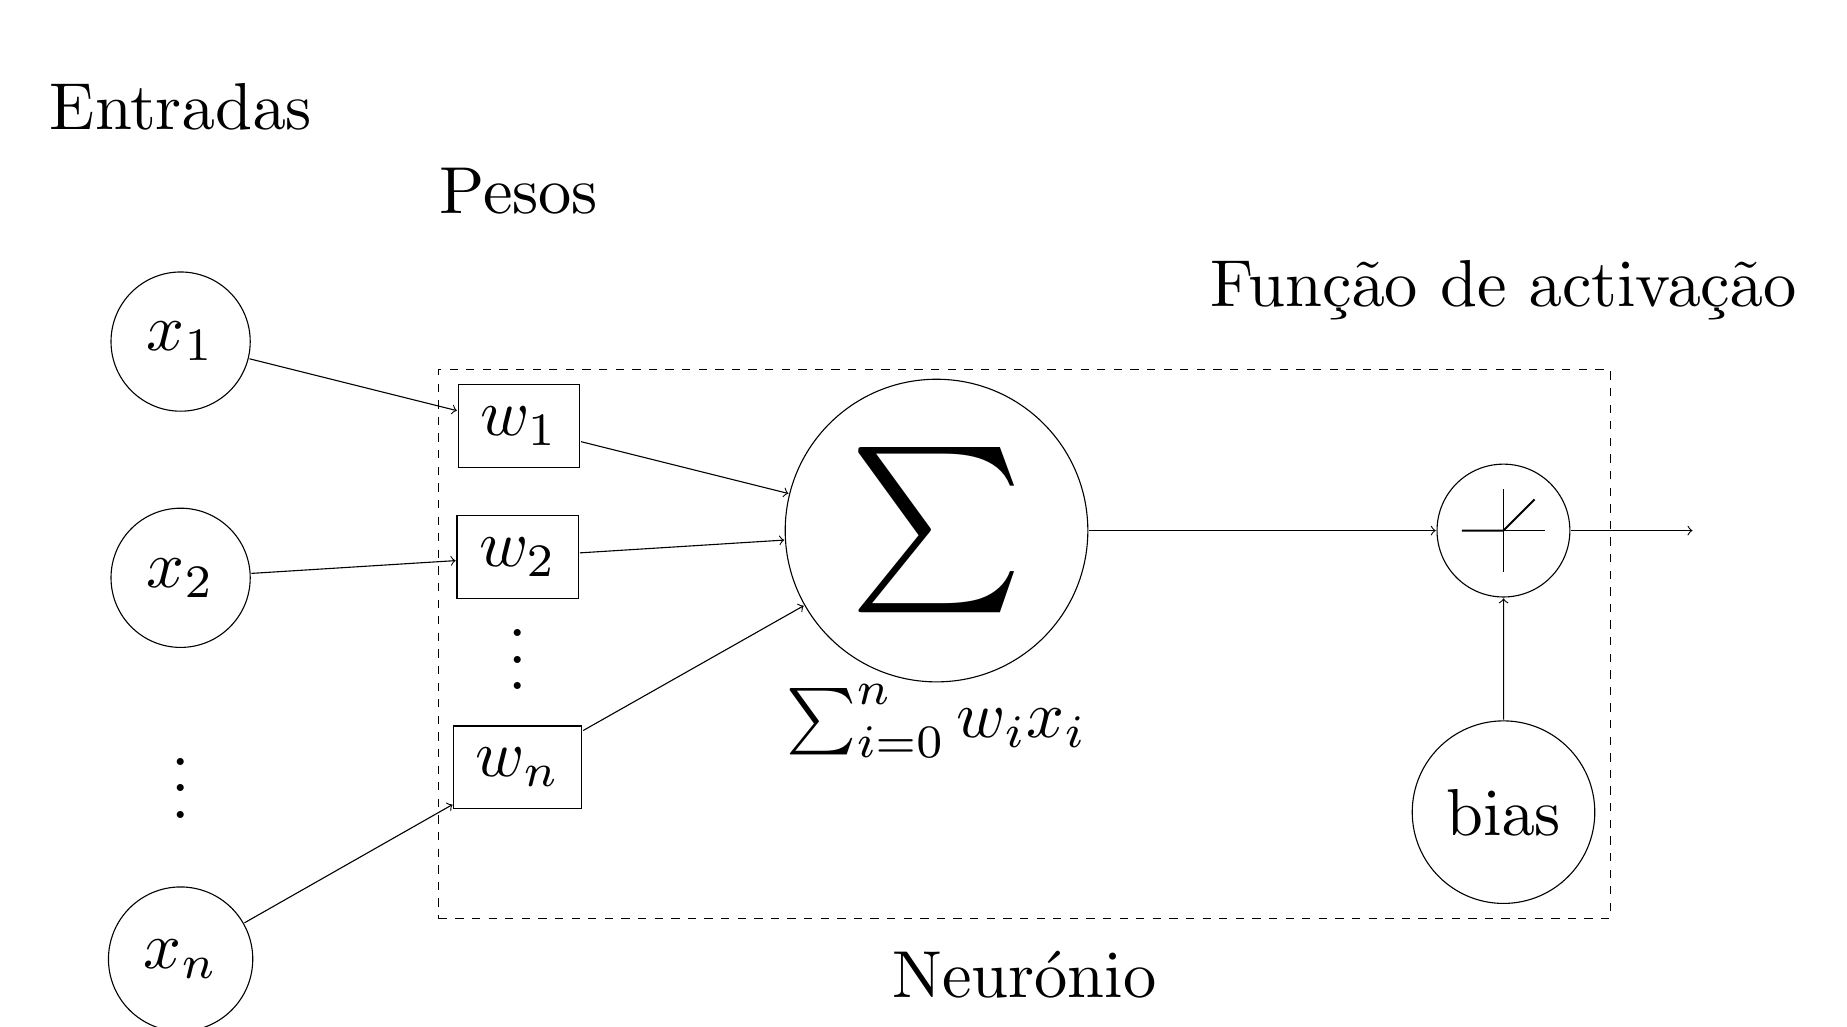
\begin{tikzpicture}[scale=2.4, transform shape]
    % Draw input nodes
    \foreach \h [count=\hi ] in {$x_2$,$x_1$}{%
          \node[input] (f\hi) at (0,\hi*1.25cm-1.5 cm) {\h};
        }
    % Dot dot dot ... x_n
    \node[below=0.62cm] (idots) at (f1) {\vdots};
    \node[input, below=0.62cm] (last_input) at (idots) {$x_n$};
    % Draw summation node
    \node[functions] (sum) at (4,0) {\Huge$\sum$};
    \node[below=0.69cm] at (sum) {$\sum_{i=0}^n w_ix_i$};
    % Draw edges from input nodes to summation node
    \foreach \h [count=\hi ] in {$w_2$,$w_1$}{%
          \path (f\hi) -- node[weights] (w\hi) {\h} (sum);
          \draw[->] (f\hi) -- (w\hi);
          \draw[->] (w\hi) -- (sum);
        }
    % Dot dot dot ... w_n
    \node[below=0.05cm] (wdots) at (w1) {\vdots};
    \node[weights, below=0.45cm] (last_weight) at (wdots) {$w_n$};
    % Add edges for last node and last weight etc
    \path[draw,->] (last_input) -- (last_weight);
    \path[draw,->] (last_weight) -- (sum);
    % Draw node for activation function
    \node[functions] (activation) at (7,0) {};
    \node[small_input, below=1cm] (bias) at (activation) {bias};
    \path[draw,->] (bias) -- (activation);

    % Place activation function in its node
    \begin{scope}[xshift=7cm,scale=1.25]
        \addaxes
        % flexible selection of activation function
        \relu
        % \stepfunc
    \end{scope}
    % Connect sum to relu
    \draw[->] (sum) -- (activation);
    \draw[->] (activation) -- ++(1,0);
    % Labels
    \node[above=1cm]  at (f2) {Entradas};
    \node[above=1cm] at (w2) {Pesos};
    \node[above=1cm] at (activation) {Função de activação};

    % Neuron
    \node[draw, dashed, fit= (w2) (last_weight) (activation) (bias), inner sep=0.5em] (square){};
    \node[below=1.5cm] at (square) {Neurónio};

\end{tikzpicture}}
	\caption{Ilustração de um neurónio. Adaptado de \cite{Haykin1999}}
	\label{fig:neuronio}
\end{figure}



\subsection{CNN\label{se:cnn_sec}}
% TODO: add cites do conv 
As Redes Neuronais Convolucionais (\gls{CNN}) diferem das \gls{FCNN} no sentido em que os filtros (neurónios) não são criados aleatoriamente, mas sim cada filtro trata de uma parte da camada de entrada. Nas convoluções é criada uma janela móvel que percorre a camada, criando um saída desse conjunto de pontos. Esta janela move-se sempre subsequentemente.\\
Esta operação é normalmente feita na dimensão (ou dimensões) em que queremos perceber padrões.\
Nos nossos dados a convolução será na dimensão temporal.\\
Se tivermos uma matriz com nove passos temporais (N,9,1), se o tamanho da janela de convolução for 3, teremos uma saída de tamanho 6 (N, 6, 1).\\
\begin{figure}[H]
	\centering
	\resizebox{\linewidth}{!}{
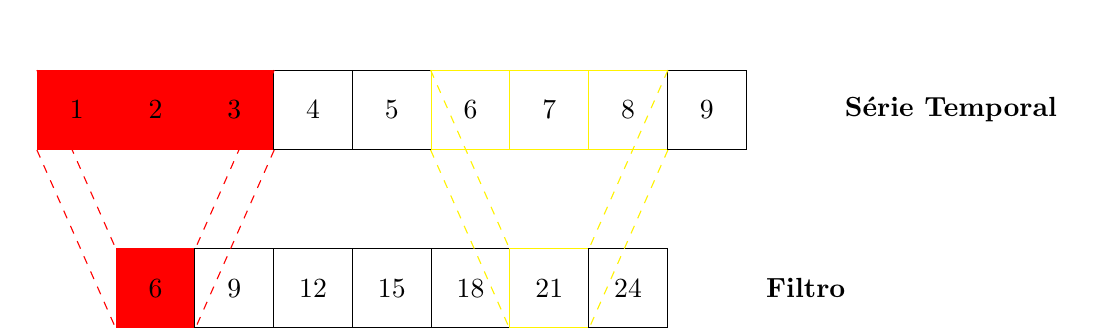
\begin{tikzpicture}
    % Time series
    \matrix (M1) [matrix of math nodes, nodes={draw, minimum size=1cm, anchor=center}, 
    column sep=-\pgflinewidth, row sep=-\pgflinewidth,
    ] {
        \node[fill=red, draw=red] (M1-1-1) {1}; & \node[fill=red, draw=red] (M1-2-1) {2};
        & \node[fill=red, draw=red] (M1-3-1) {3}; &
        4 & 5 & \node[draw=yellow] (M1-6-1) {6}; & \node[draw=yellow] (M1-7-1) {7};
        & \node[draw=yellow] (M1-8-1) {8}; & 9 \\
    };
    
    % Kernel
    \matrix (M2) [below=of M1, matrix of math nodes, nodes={draw, minimum size=1cm, anchor=center}, 
    column sep=-\pgflinewidth, row sep=-\pgflinewidth,
    ] {
        \node[fill=red, draw=red] (M2-1-1) {6}; & 9 & 12 & 15 & 18 & \node[draw=yellow] (M2-5-1) {21}; & 24 \\
    };

    \draw[dashed, red] (M1-1-1.north west) -- (M2-1-1.north west);
    \draw[dashed, red] (M1-3-1.north east) -- (M2-1-1.north east);
    \draw[dashed, red] (M1-1-1.south west) -- (M2-1-1.south west);
    \draw[dashed, red] (M1-3-1.south east) -- (M2-1-1.south east);

    \draw[dashed, yellow] (M1-6-1.north west) -- (M2-5-1.north west);
    \draw[dashed, yellow] (M1-8-1.north east) -- (M2-5-1.north east);
    \draw[dashed, yellow] (M1-6-1.south west) -- (M2-5-1.south west);
    \draw[dashed, yellow] (M1-8-1.south east) -- (M2-5-1.south east);

    
    % Titles
    \node [right=1cm, align=center, font=\bfseries] at (M1.east) {Série Temporal};
    \node [right=1cm, align=center, font=\bfseries] at (M2.east) {Filtro};
    \end{tikzpicture}}
	\caption{Ilustração da operação de Convolução}
	\label{fig:conv_layer1D}
\end{figure}

Anteriormente ignoramos o número de filtros. Mas as convoluções criam o número pedido de filtros para cada janela temporal. Aqui cada filtro vai funcionar como na camada \gls{FCNN}, onde cada um começa com uma operação pseudo aleatória. Esta operação normalmente é feita na dimensão dos atributos.\\
Ou seja, a quantidade de filtros que esta camada irá produzir por convolução.\\
Se tivermos a mesma entrada que anteriormente mas com 4 atributos (N, 9, 4), e se definir o número de filtros para 2 teremos uma saída (N, 6, 2).\\
Ou seja, dois filtros por cada janela temporal.\\


\begin{figure}[H]
	\centering
	\resizebox{\linewidth}{!}{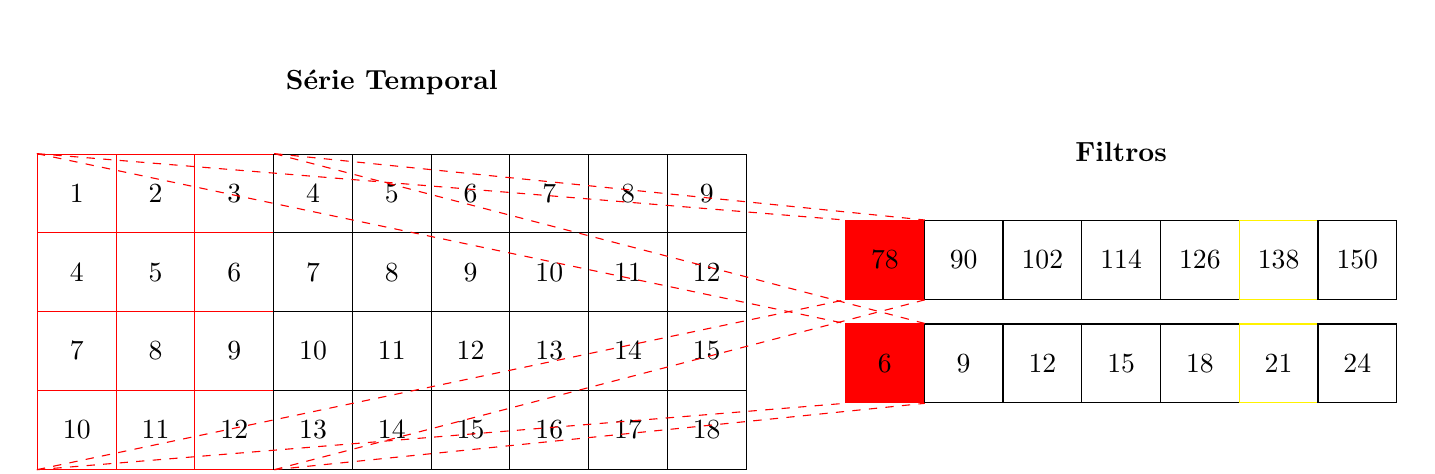
\begin{tikzpicture}[scale=2]
    \matrix (M1) [matrix of math nodes, nodes={draw, minimum size=1cm, anchor=center}, 
    column sep=-\pgflinewidth, row sep=-\pgflinewidth,]
{
    \node[draw=red] (M1-1-1) {1}; & \node[draw=red] (M1-1-2) {2}; & \node[draw=red] (M1-1-3) {3}; & 4 & 5 & 6 & 7 & 8 & 9\\
    \node[draw=red] (M1-2-1) {4}; & \node[draw=red] (M1-2-2) {5}; & \node[draw=red] (M1-2-3) {6}; & 7 & 8 & 9 & 10 & 11 & 12\\
    \node[draw=red] (M1-3-1) {7}; & \node[draw=red] (M1-3-2) {8}; & \node[draw=red] (M1-3-3) {9}; & 10 & 11 & 12 & 13 & 14 & 15\\
\node[draw=red] (M1-4-1) {10}; & \node[draw=red] (M1-4-2) {11};
& \node[draw=red] (M1-4-3) {12}; & 13 & 14 & 15 & 16 & 17 & 18\\
};

\matrix (M2) [matrix of math nodes, nodes={draw, minimum size=1cm, anchor=center}, 
column sep=-\pgflinewidth, row sep=0.3cm,
    right=of M1]
{
    \node[fill=red, draw=red] (M2-1-1) {78}; & 90 & 102 & 114 & 126 & \node[draw=yellow] (M2-1-5) {138}; & 150 \\
    \node[fill=red, draw=red] (M2-2-1) {6}; & 9 & 12 & 15 & 18 & \node[draw=yellow] (M2-2-5) {21}; & 24 \\
    };

% Titles
\node [above=0.5cm, align=center, font=\bfseries] at (M1.north) {Série Temporal};
\node [above=0.5cm, align=center, font=\bfseries] at (M2.north) {Filtros};
 
\draw[dashed, red] (M1-1-1.north west) -- (M2-1-1.north west);
\draw[dashed, red] (M1-1-1.north west) -- (M2-2-1.north west);

\draw[dashed, red] (M1-1-3.north east) -- (M2-1-1.north east);
\draw[dashed, red] (M1-1-3.north east) -- (M2-2-1.north east);

\draw[dashed, red] (M1-4-1.south west) -- (M2-1-1.south west);
\draw[dashed, red] (M1-4-1.south west) -- (M2-2-1.south west);


\draw[dashed, red] (M1-4-3.south east) -- (M2-1-1.south east);
\draw[dashed, red] (M1-4-3.south east) -- (M2-2-1.south east);



% TODO: add legenda em pequeno
%\node [right=1cm, align=center, font=\bfseries] at (matrix1.west) {Atributos};
%\node [right=1cm, align=center, font=\bfseries] at (matrix1.south) {tempo};


\end{tikzpicture}}
	\caption{Ilustração da camada de Convolução}
	\label{fig:conv_layer}
\end{figure}

As convoluções podem realizar as operações em mais dimensões, é comum usar 2D para imagens, e 3D para vídeos. Neste trabalho apenas trabalhamos com convoluções 1D.\\

\subsubsection{UNET\label{se:unet_sec}}

Um desenho especial de \gls{CNN}, normalmente usando em modelação de imagens, e primeiro proposto em \cite{Shelhamer2014}, a arquitectura UNET passa por criar uma rede de expansão dos filtros, usando convoluções, e de seguida uma rede de contracção dos mesmo, até aos tamanhos pretendidos.\\
Nas suas ligações UNET junta informação de filtros passados (não de nível temporal mas de rede neuronal) para realçar informação já trabalhada, e assim identificar padrões de vários contextos diferentes.\\
É chamada assim pois é uma rede (NET) que forma um U na sua expansão, contracção e ligações entre estes.\\
Em cada camada de encoding vai usando convulucões para criar novos filtros e diminuir a dimensionalidade, enquanto que na fase de decoding vai usar convoluções para aumentar a dimensionalidade e diminuir o número de filtros, adicionando a camada decoder de tamanho análogo.\\

\begin{figure}[H]
	\centering
	\resizebox{\linewidth}{!}{\begin{tikzpicture}[ node distance = 2cm, auto, block/.style={ rectangle, draw, align=center, minimum width=2cm, minimum height=1cm }, line/.style={ draw, -latex' } ]
    % Encoder (Contracting Path)
    \node [block] (input) {Input};
    \node [block, below right=of input, xshift=-2cm] (enclayer1) {Enconding1};
    \node [block, below right=of enclayer1, xshift=-1.8cm] (enclayer2) {Enconding2};
    \node [block, below right=of enclayer2, xshift=-1.6cm] (enclayer3) {Enconding3};
    % (None, 168, 18) 
    
    \node [block, below right=of enclayer3] (up1) {Enconding4};
    
    % Decoder (Expanding Path)
    \node [block, above right=of up1] (declayer1) {Decoding1};
    \node [block, above right=of declayer1, xshift=-1.6cm] (declayer2) {Decoding2};
    \node [block, above right=of declayer2, xshift=-1.8cm] (declayer3) {Decoding3};
    \node [block, above right=of declayer3, xshift=-2cm] (output) {Output};
    
    % Skip Connection
    % \draw [line] (pool1) -- ++(0,-1) -| (up1);
    
    % Connections
    \draw [line] (input) -- (enclayer1);
    \draw [line] (enclayer1) -- (enclayer2);
    \draw [line] (enclayer2) -- (enclayer3);
    \draw [line] (enclayer3) -- (up1);
    \draw [line] (up1) -- (declayer1);
    
    
    \draw [line] (declayer1) -- (declayer2);
    \draw [line] (declayer2) -- (declayer3);
    \draw [line] (declayer3) -- (output);
    
    
    \draw [line] (input) -- (output);
    \draw [line] (enclayer1) -- (declayer3);
    \draw [line] (enclayer2) -- (declayer2);
    \draw [line] (enclayer3) -- (declayer1);
    
    
    \end{tikzpicture}}
	\caption{Ilustração uma rede UNET.}
	\label{fig:unet_graph}
\end{figure}


\subsection{RNN\label{se:rnn_sec}}

As Redes Neuronais Recorrentes (RNN) são projetadas para processar sequências de dados, onde a ordem dos elementos é importante. Elas funcionam passando informações de um neurónio para outro em uma cadeia, o que permite que cada neurónio seja influenciado pelo estado anterior da rede.\\
Isso é feito através de loops internos que permitem à rede "lembrar" informações de etapas anteriores. No entanto, as RNNs enfrentam dificuldades ao tentar lembrar informações de longo prazo, devido ao problema conhecido como desvanecimento do gradiente, onde os gradientes se tornam muito pequenos e impedem a atualização eficaz dos pesos da rede.\\

\subsubsection{LSTM\label{se:lstms_sec}}

As redes \gls{LSTM} são um tipo especial de RNN projetado para superar os problemas de memória de longo prazo encontrados nas RNNs. Isto é conseguido através de uma estrutura de célula que mantém informações ao longo do tempo, permitindo que a rede lembre detalhes importantes mesmo após muitos passos no tempo.\\
As \gls{LSTM}s usam mecanismos de portão para controlar o fluxo de informações, permitindo que elas ignorem informações irrelevantes e mantenham as informações relevantes. Isso torna-as particularmente eficazes em tarefas que exigem o entendimento de dependências de longo prazo em dados sequenciais.\\


O uso de \gls{LSTM} para previsões é uma área comum, mas aqui é seguido através das ideas partilhas em \cite{Hewamalage2021}, e reforçado pelo uso em previsões energéticas demonstados em \cite{Costa2022} \\


\subsection{Transformer\label{se:transformer_sec}}

Os Transformers são um tipo de arquitetura de modelo que utiliza mecanismos de atenção para pesar a importância de diferentes partes de um dado de entrada, primeiro apresentado em \cite{Vaswani2017}.\\
Em vez de processar os dados sequencialmente, como as RNNs, os Transformers processam todos os elementos do dado de entrada simultaneamente. Isso é feito através de um mecanismo de atenção que calcula uma pontuação de atenção para cada par de elementos no dado de entrada, indicando quão relevante um elemento é para o outro. Essas pontuações de atenção são então usadas para ponderar a contribuição de cada elemento ao resultado final. \\
Isso permite aos Transformers capturar dependências de longo alcance nos dados de forma eficiente, tornando-os extremamente eficazes para tarefas de processamento de linguagem natural, como tradução automática e sumarização de texto.\\
% TODO: ref para cahtgpt e dall-e e assim
Este tipo de desenho é a base para os modelos generativos mais conhecidos como o chatGPT para linguagem ou o Dall-E para imagens.\\



\label{ch:contexto}
% Dados

\newpage
\thispagestyle{plain}
\chapter{Estudo 1: Estimativa do parâmetro $\rho$ da fórmula da REN}



Para responder a primeira questão estudou-se o comportamento do parâmetro p na equação publicada pela \gls{REN} para a Banda de Regulação Secundária a Subir:

\begin{equation} \label{eq:BRREN} 
    BR = \rho \times \sqrt{a \times  L_{max} + b^{2}} - b 
\end{equation}
onde:
\begin{itemize}
  \item $BR$: Banda de Reserva  de regulação secundária necessária (MW).
  \item $\rho$: Paramêtro horário.
  \item $a$ e $b$: Coeficientes empiricos, $a$=10MW e $b$=150MW .
  \item $L_{max}$: Pico máximo de consumo (MW).
\end{itemize}

Aqui queremos descobrir qual o valor do parâmetro $\rho$ (por hora do dia) que melhor nos descreve os dados reais. Para isso estudamos os valores reais usados para a Banda de Reserva, os valores resultantes da proposta de $\rho$  em \cite{Carneiro2016} e os valores resultados do estudo aqui proposto. Aproximar o parâmetro $\rho$  utilizando os dados históricos. \\
Todos os dados necessários são disponibilizados pelo operador do sistema no \href{https://mercado.ren.pt/PT/Electr}{site da \gls{REN}}, com exceção do consumo máximo expectável. Este parâmetro é então substituído pelo consumo real, como uma aproximação à formulação indicada previamente.\\
Os dados estudados contêm entradas horárias desde 2010 até ao fim de 2018. Com as seguintes variáveis:\\

\begin{table}[H] \centering \caption{Dados REN} \begin{tabular}{ll}
\toprule
Nome & Unidades \\
\midrule
Necessidade Banda Subir [MW] & MW \\
Necessidade Banda Descer [MW] & MW \\
Consumo [MWh] & MWh \\
\bottomrule
\end{tabular}
 \end{table}

Na equação \ref{eq:BRREN} BR equivale à soma de BANDA SUBIR e BANDA DESCER, onde aqui é sempre considerado que Banda a subir são $\frac{2}{3}$ da Banda de Reserva total e a Banda a descer é o restante $\frac{1}{3}$. \\
Aqui iremos aplicar o mapa de parâmetro $\rho$ apresentado em \cite{Carneiro2016} na formula \ref{eq:BRREN} para o cálculo da Banda de Reserva Carneiro2016 como benchmark. \\

\begin{table}[H] \centering \caption{Valores de $\rho$ apresentado em \cite{Carneiro2016}} \begin{tabular}{ll}
\toprule
Hora & $\rho$ \\
\midrule
1/2/8/9/24 & 1,6 \\
3/7/10/11/19/20 & 1,4 \\
4 & 1,3 \\
5/6/12/13/14/15/16/17/18/21/22/23 & 1,2 \\
\bottomrule
\end{tabular}
 \end{table}


Por outro lado, usando os dados de consumo real, calculamos o $\rho$ ideal para cada entrada, de onde estudamos a melhor normalização dos mesmos para cada hora. \\
O cálculo deste $\rho_{proposto}$ é apenas a utilização da fórmula \ref{eq:BRREN} mas em função de $\rho$ : \\

\begin{equation} \label{eq:rhoproposed} 
    \rho  = \frac{(BR + b)}{\sqrt{a \times L_max + b^{2}}}
\end{equation}


Arredondando o $\rho_{proposto}$ a uma casa decimal, podemos verificar que o histograma das diferentes propostas difere bastante. Sendo que esta apresenta uma curva de distribuição normal. \\


\begin{figure}[H]
    \centering
    \includegraphics[width=\textwidth]{plots/Histograma_parametro_p.png}
    \caption{Histograma $\rho$}
  \end{figure}


Olhando as distribuições por hora: \\

\begin{figure}[H]
    \centering
    \includegraphics[width=\textwidth]{plots/Valor_do_parametro_p_hora.png}
    \caption{Valor do paramêtro $\rho$ (hora)}
  \end{figure}

O $\rho_{proposto}$ apresenta um grande variabilidade em todas as horas, embora de notar que em todas tem um maior peso perto da mediana. O $\rho$ de comparação embora sempre dentro da distribuição note-se que cai quase sempre em zonas com pouco peso nestes dados históricos. \\
Calculamos $\rho$ possiveis para proposta final usando as seguintes aproximações: média, mediana, e média ponderada ao consumo, e à banda. \\

As distribuições por hora são as seguintes:

\begin{figure}[H]
    \centering
    \includegraphics[width=\textwidth]{plots/Comparação_de_p_propostos_por_hora.png}
    \caption{Histograma $\rho$}
\end{figure}

Todas seguem um percurso semelhante ao longo do dia, o qual também pode ser extrapolado para Carneiro2016. A média e mediana destacam-se seguindo muito parecidas, enquanto que as ponderadas também parecidas entre elas são bastante mais discretas. \\
Para a escolha da normalização deste parâmetro à Hora, estudou-se o erro entre a Banda Reserva calculada através das normalizações e a Banda Reserva disponível nos dados. \\


\begin{figure}[H]
    \centering
    \includegraphics[width=\textwidth]{plots/Comparação_das_metricas_de_Erro.png}
    \caption{Histograma $\rho$}
\end{figure}


\begin{table}[H]
    \caption{Erros de Banda de Reserva por método de normalização $rho$}    
    \resizebox{\linewidth}{!}{\begin{tabular}{lrrrr}
\toprule
 & MAE & RMSE & MedianAE & MAPE \\
Normalização &  &  &  &  \\
\midrule
Carneiro2016 & 49.55 & 60.52 & 44.65 & 29.36 \\
média & 14.67 & 19.87 & 11.18 & 8.80 \\
mediana & 14.03 & 20.36 & 8.15 & 8.44 \\
média ponderada consumo & 15.76 & 21.91 & 10.32 & 9.30 \\
média ponderada banda & 16.19 & 22.23 & 11.30 & 9.73 \\
\bottomrule
\end{tabular}
}
    \end{table}


A normalização com erros mais baixos é a mediana. Com um erro médio (de todo o histórico) para o consumo real de 11.51\% o que comparando com o benchmark de 18.70\% é uma melhoria  bastante considerável. \\
Comparando as bandas calculadas a uma média em cada hora: \\


\begin{figure}[H]
    \centering
    \includegraphics[width=\textwidth]{plots/média_historica_de_banda_de_reserva.png}
    \caption{Média historica de Banda de Reserva}
\end{figure}

Podemos ver que em termos de média horária, a Banda de Reserva calculada através do $\rho_{proposto}$ apresenta quase uma sobreposição por inteiro ao valor médio real. \\

Retiramos as médias dos erros percentuais e podemos observar: \\

\begin{figure}[H]
    \centering
    \includegraphics[width=\textwidth]{plots/erro_médio_por_hora_banda_de_reserva.png}
    \caption{Erro médio por hora Banda de Reserva}
\end{figure}

Em termos de média diária o erro pelo método proposto está bem abaixo da margem de erro do 5\% na banda, em todas as horas. E na outra tese apenas 10\% cai dentro dessa margem de erro. \\

Como tal o $\rho_{proposto}$ a partir do estudo dos dados  históricos é: \

\begin{table}[H] \centering \caption{Valores de $\rho$ propostos} \begin{tabular}{lr}
\toprule
Hora & \rho \\
\midrule
0 & 1.252829 \\
1 & 1.256717 \\
2 & 1.240812 \\
3 & 1.186709 \\
4 & 1.128716 \\
5 & 1.107658 \\
6 & 1.106000 \\
7 & 1.175438 \\
8 & 1.225913 \\
9 & 1.224505 \\
10 & 1.175051 \\
11 & 1.166680 \\
12 & 1.135893 \\
13 & 1.128339 \\
14 & 1.141243 \\
15 & 1.141133 \\
16 & 1.129779 \\
17 & 1.132071 \\
18 & 1.129844 \\
19 & 1.173754 \\
20 & 1.179720 \\
21 & 1.135143 \\
22 & 1.146282 \\
23 & 1.160048 \\
\bottomrule
\end{tabular}
 \end{table}


% \begin{table}[H]
%     \caption{Valores de $\rho$ propostos}    
%     \resizebox{\linewidth}{!}{\begin{tabular}{lr}
\toprule
Hora & \rho \\
\midrule
0 & 1.252829 \\
1 & 1.256717 \\
2 & 1.240812 \\
3 & 1.186709 \\
4 & 1.128716 \\
5 & 1.107658 \\
6 & 1.106000 \\
7 & 1.175438 \\
8 & 1.225913 \\
9 & 1.224505 \\
10 & 1.175051 \\
11 & 1.166680 \\
12 & 1.135893 \\
13 & 1.128339 \\
14 & 1.141243 \\
15 & 1.141133 \\
16 & 1.129779 \\
17 & 1.132071 \\
18 & 1.129844 \\
19 & 1.173754 \\
20 & 1.179720 \\
21 & 1.135143 \\
22 & 1.146282 \\
23 & 1.160048 \\
\bottomrule
\end{tabular}
}
%     \end{table}

Em relação a perdas por arredondamento, apresento o resultado dos erros por arrendamento em cada um da casas possíveis, concluindo que até à primeira casa decimal, pode ser feito arredondamento do parâmetro $\rho$, sem influenciar muito o erro: \\


\begin{figure}[H]
    \centering
    \includegraphics[width=\textwidth]{plots/Erro_médio_por_hora_Banda_de_Reserva_Arredondamento.png}
    \caption{Erro médio por hora Banda de Reserva (Arredondamento)}
\end{figure}



Neste estudo podemos comprovar que usando um $\rho$ extrapolado dos dados históricos, e um $L_{max}$ sendo o consumo real e não o consumo máximo calculado, os erros médios por hora ficam abaixo dos 5\%.\\ \label{ch:estudo_1}

\newpage
\thispagestyle{plain}
% \part{Dimensionamento dinâmico da potência alocada na reserva secundária}

\chapter{Dados}
\section{Dados Utilizados\label{se:dadosestudo}}

Os dados em estudo são do mercado energético espanol, retirados do site da \href{https://www.esios.ree.es/es}{\gls{ESIOS}}.


\begin{table}[H]
    \caption{Indicadores retirados do site da ESIOS}    
    \resizebox{\linewidth}{!}{\csvautotabular{tabelas/indicators_metadata.csv}}
\end{table}


\subsection{Aquisição dos Dados}

No ambito da automatização destes dados foi modificado o repositorio \href{https://github.com/SanPen/\gls{ESIOS}}{\gls{ESIOS}} para ser usado como uma biblioteca de python, aberta, em pypi.\par
Sendo uma ferramenta mais facilmente acessivel para a extrair dados do mercado espanhol, \href{https://pypi.org/project/pyesios/}{pyesios}.\par
No âmbito de automatizar o processo, foram feitas contribuições a esta ferramenta para tornar mais acessível, e uma ferramenta aberta de python.\par


\thispagestyle{plain}

\section{Estudo dos dados}

Os dados que proponho a prever são os de Energia Usada na Banda de Reserva Secundária, tanto a subir como a descer: "UpwardUsedSecondaryReserveEnergy","DownwardUsedSecondaryReserveEnergy".\\



\begin{figure}[H]
  \centering
  \includegraphics[width=\textwidth]{plots/consumo_originais.png}
  \caption{Serie Temporal dos dados alvo}
  \label{fig:targettimeseries}
\end{figure}


Para termos uma melhor percepção dos mesmos segue algumas janelas temporais mais pequenas.

\begin{figure}[H]
  \centering
  \includegraphics[width=\textwidth]{plots/target_timeseries_windows.png}
  \caption{Janelas Temporais dos dados alvo}
  \label{fig:targettimeserieswindows}
\end{figure}


Estas mostram claramente que ambos os atributos mantêm um comportamento tanto discreto, como linear, isto é, que ou existe algum valor, ou é zero, e se existe valor este tem comportamento linear.\\
A distribuição destes dados é claramente exponencial. O que é importante para a escolha de alguns parâmetros na modelação. \\

		
\begin{figure}[H]
  \centering
  \includegraphics[width=\textwidth]{plots/target_histograms.png}
  \caption{Frequência dos dados alvos}
  \label{fig:targethistograms}
\end{figure}


\subsection{Correlações}

Os modelos vão depender bastante de correlação entre variáveis.

Nesta secção queremos tentar identificar se há visiveis relações entre as variáveis, e se há relações temporais  visiveis nas colunas alvo.


\subsubsection{Correlações entre atributos}


\begin{figure}[H]
  \centering
  \includegraphics[width=\textwidth]{plots/feature_correlation.png}
  \caption{Correlação entre atributos}
  \label{fig:featurecorrelation}
\end{figure}

Esta figura apresenta a dispersão de valores entre a energia usada, primeiras três linhas a energia para cima e as seguintes a energia para baixo, e os outros atributos presentes.\\
As correlações entre variáveis parecem muitos escassas, o que apresenta já que a previsão destes dados usando estas variáveis vai ser um problema difícil.\\
Por norma é feito uma seleção de atributos baseado nestas correlações, eliminando assim os atributos que ajudam menos, ou até prejudicam os modelos.\\
Segue os valores de correlação onde podemos ver numericamente que existe muito pouca correlação entre os atributos. Onde a primeira coluna são os valores de correlação para a energia usada a subir e a segunda coluna as correlações da energia usada a descer.\\

\begin{figure}[H]
  \centering
  \includegraphics[width=\textwidth]{plots/correlation_heatmap.png}
  \caption{Valores de correlação entre atributos}
  \label{fig:correlationheatmap}
\end{figure}

\subsubsection{Correlações Temporais}

\begin{figure}[H]
  \centering
  \includegraphics[width=\textwidth]{plots/autocorrelation.png}
  \caption{Autocorrelação Temporal}
  \label{fig:autocorrelation}
\end{figure}

A autocorrelação, em ambos os alvos, é mais forte nas 3 horas mais próximas, e nos pontos com diferença de 12 e 24 horas. \\
É de notar que estes valores são baixos, prometendo já também uma baixa regressividade temporal. \\
Os melhores saltos temporais e suas correlações são mostradas na tabelas em baixo:\\


\begin{table}[H]
  \caption{Autocorrelação Temporal}    
  \resizebox{\linewidth}{!}{\begin{tabular}{lllllllllll}
\toprule
\midrule
\multirow[t]{2}{*}{UpwardUsedSecondaryReserveEnergy} & horas & 1 & 2 & 24 & 23 & 25 & 168 & 144 & 192 & 48 \\
 & rácio & 0.44 & 0.24 & 0.22 & 0.19 & 0.19 & 0.17 & 0.16 & 0.16 & 0.16 \\
\cline{1-11}
\multirow[t]{2}{*}{DownwardUsedSecondaryReserveEnergy} & horas & 1 & 2 & 24 & 23 & 25 & 168 & 144 & 192 & 48 \\
 & rácio & 0.43 & 0.22 & 0.25 & 0.20 & 0.19 & 0.21 & 0.19 & 0.20 & 0.19 \\
\cline{1-11}
\bottomrule
\end{tabular}
}
  \label{tab:tempcorr}
  \end{table}

Outro ponto a denotar é que os objectos não têm um comportamento completamente linear, i.e., parece existir um comportamento discreto na questão ser alocado ou não esta reservas secundárias, e caso seja alocado, aí existir alguma linearidade. \\
Logo qualquer tipo de modelação terá de resolver primeiramente este problema. \\
Estas relações mostram que em termos de atributos usados vai ser um desafio complicado para qualquer tipo de modelo. \\
No âmbito desta dissertação queremos verificar a qualidade das previsões usando estes mesmo atributos, logo, não será feita seleção dos mesmos. \\
A nível da relação temporal, a maior parte dos modelos que iremos testar aplica um janela na dimensão temporal, usando todos os valores nessa janela, e aplicando os pesos nessas distâncias que mais se enquadram. Logo também não é relevante escolher apenas as distâncias temporais com maior correlação, pois os modelos vão fazer essa pesagem. \\


 \label{se:dadoscrus}



\thispagestyle{plain}



\section{Tratamento dos dados}

\textbf{Normalização} \par
A normalização foi deixada por ser aprendida nos modelos, sendo que todos têm como segunda camada, uma de normalização.\par

\textbf{Limpeza} \par

Podemos ver pelos gráficos seguintes que a existem alguns outliers, sendo estes definidos como 3 desvios padrão de distância à média.\par
Estes gráficos mostram também que existe uma variação do que são os valores normais de cada atributo a nível temporal. Logo um método de limpeza não se poderia basear apenas numa definição geral de outliers, mas teria de ser feito em janelas temporais.\par
Pelo mesmo argumento e visto que os outliers fazem parte do que queremos também descobrir, não é aplicada nenhum método de remoção dos mesmo, sendo os dados passados a cru para os modelos.\par


\begin{figure}[H]
  \centering
  \includegraphics[width=\textwidth]{plots/Outliers_3stds.png}
  \caption{Outliers}
\end{figure}

Outra análise desta variação dos atributos a nível temporal leva-nos a que qualquer divisão dos dados para treino e teste deva levar as variações em consideração. Isto sendo que o treino deve ter representatividade de todas, ou maior parte, das condições diferentes.\par


\textbf{Dados em falta (Missing Data)}

Estudemos também o caso de dados em falta. Alguns destes atributos têm certas entradas vazias, e como podemos ver alguns não têm alguns anos inteiros.\par
Como queremos usar o máximo de dados possíveis iremos usar técnicas de imputing nesses dados.\par
Podemos ver que temos dados em falta de vários anos, em três atributos, e um tem algumas horas esporádicas em falta nos primeiros anos.\par

\begin{figure}[H]
  \centering
  \includegraphics[width=\textwidth]{plots/missing_data.png}
  \caption{Dados em falta}
\end{figure}

Vamos aplicar o método experimental \href{https://scikit-learn.org/stable/modules/generated/sklearn.impute.IterativeImputer.html}{IterativeImputer} da biblioteca de python \href{https://scikit-learn.org/stable/index.html}{sklearn}.\par
Este metodo é baseado nos trabalhos de \cite{vanBuuren2011} e de \cite{Buck1960}.\par
Por ultimo foi adicionado ao dados mais atributos, sendo eles todos de cariz temporal. É adicionado atributos correspondentes à hora, ao dia do ano, ao dia da semana, ao dia do mês, mês, ano.\par

 \label{se:tratamentodados}

\subsection{Dados de treino}

Após o tratamento apresentado as estatísticas gerais dos dados usados para treinar o modelo são:

\begin{table}[H]
    \caption{Dados de Treino}    
    \resizebox{\linewidth}{!}{\begin{tabular}{lrrrr}
\toprule
 & média & desvio padrão & min & max \\
\midrule
DownwardUsedSecondaryReserveEnergy & 168.18 & 199.23 & 0.00 & 1721.40 \\
SecondaryReserveAllocationAUpward & 665.98 & 150.88 & 399.00 & 958.00 \\
SecondaryReserveAllocationADownward & 554.50 & 131.06 & 312.00 & 956.00 \\
UpwardUsedSecondaryReserveEnergy & 160.82 & 193.09 & 0.00 & 1654.80 \\
WindD+1DailyForecast & 5881.14 & 3480.52 & 66.13 & 20879.30 \\
PhotovoltaicD+1DailyForecast & 1676.31 & 2745.51 & 0.00 & 14925.30 \\
DemandD+1DailyForecast & 27933.38 & 4488.71 & 14170.00 & 41799.66 \\
TotalBaseDailyOperatingSchedulePBFGeneration & 27250.40 & 4608.74 & 13470.50 & 42707.60 \\
BaseDailyOperatingSchedulePBFSolarPV & 1737.79 & 2850.91 & 0.00 & 16358.90 \\
BaseDailyOperatingSchedulePBFWind & 6588.28 & 3637.80 & 308.60 & 21619.60 \\
BaseDailyOperatingShedulePBFTotalBalanceInterconnections & 266.26 & 2169.01 & -7817.00 & 6858.50 \\
\bottomrule
\end{tabular}
}
    \end{table}
 \label{ch:estudo_2}


% Arquiteturas a estudar
\newpage
\thispagestyle{plain}
\input{Capitulos/Tese-6-Arquitecturas_de_Modelos}\label{ch:arch}
% Ferramentas
\newpage
\thispagestyle{plain}
\chapter{Ferramentas}

\section{\href{https://github.com/alquimodelia/alquimodelia}{Alquimodelia}\label{se:alquimodelia}}


Com o propósito de desenvolver este estudo, e deixar ferramentas para a replicação do mesmo, foi criado uma biblioteca em python para desenhar as arquitecturas em estudo.\\

\subsection{Construtor de modelos}

Seguindo as arquitecturas descritas anteriormente esta ferramenta constrói os modelos automaticamente, sendo que precisamos apenas de fornecer os parâmetros variáveis. Permitindo assim um fácil teste de vários tipo de modelos, não tendo de reescrever código para cada um deles.\\

\subsection{\href{https://github.com/alquimodelia/alquitable/blob/main/alquitable/generator.py}{Gerador de dados}}

O gerador construido trata da formatação dos dados para entrada nos modelos. Formatação esse que se baseia nos valores de janelas temporais a usar, e na divisão treino/teste.\\
Esta ferramenta agrega os dados em tensores de formato \textit{(N, t, a)}, onde \textit{N} é o número de casos, \textit{t} é a janela temporal, e \textit{a} é o número de atributos.\\
A ferramenta permite também definir o tempo de salto entre cada entrada.\\
Usando como exemplo uma janela temporal de 168 (horas, uma semana) para treino, e 24 (horas) para o alvo. Com um salto temporal de 1 a primeira entrada teria como treino as primeiras 168 horas dos dados, e como alvo as 24 horas consequentes. A segunda entrada seria a partir da segunda hora dos dados, e assim consecutivamente. Para um caso em que o tempo de salto seria 24, a primeira entrada mantinha-se, mas a segunda começaria 24 horas depois, e não apenas uma.\\

Como estamos também a lidar com dados desfasados, o gerador atribui este desfasamento em atributos a especificar. No caso em estudo temos que os atributos são de \gls{DA}, logo estão desfasados 24 horas. O que implica termos de aplicar este desfasamento nos dados que não são \gls{DA}, nomeadamente os dados alvo. Esta propriedade permite também o fácil uso da ferramenta noutros dados desfasados, como as previsões a 3 ou 8 horas.\\

\section{\href{https://github.com/alquimodelia/MuadDib}{MuadDib}\label{se:muaddib}}

Esta ferramenta criada para desenvolver as experiências desta dissertação, permite ao utilizador apenas com os dados que quer utilizar e a especificação das métricas pretendidas, facilmente ter um modelo optimizado para os seus dados e problema.\\
Ao usar a ferramenta o utilizador consegue testar vários modelos e hiper parametrizações diferentes mas mantendo a necessidade de escrever código ao mínimo.\\
\label{ch:ferramentas}
\newpage
\thispagestyle{plain}
\input{Capitulos/Tese-8-Metricas}\label{ch:metricas}

% Métodos
\newpage
\thispagestyle{plain}
\chapter{Métodos}

A todas as experiências foram aplicadas as métricas apresentadas, excepto no benchmark onde teríamos métricas de comparação a ele próprio.\par
Para a escolha de melhor modelo dentro das experiências foi escolhido o modelo que melhor resultados apresentou para a métrica em questão. Sendo esta o GPD $Norm^{2}$ enquanto não encontramos uma melhoria tanto na alocação em falta como na em demasia, ao que se seguida foi usado o GPD Positivo.\par
No caso das Redes Neuronais a hiper parametrização foi feita também deste modo, sendo que primeiro se encontrou uma hiper parametrização adequada aos dados, usando uma arquitetura simples e só depois com essa configuração foi feita a experiência  nas várias arquiteturas.\par
O objectivo é conseguir um modelo que tenha a uma Alocação Total em Falta e Alocação Total em Demasia menor que o Benchmark, dentro dos anos 2019 a 2022. Logo em termos de métricas um GPD Positivo mais elevado possível.\par

\thispagestyle{plain}
\section{Estatisticos}

Em estatística conseguimos encontrar vários métodos de estudo de séries temporais. Estes métodos são normalmente usados como primeira abordagem para fazer previsões.\\
Estes modelos podem ser auto-regressivos (\gls{AR}), onde vão fazer previsões baseados num número (p) de dados anteriores. Estes modelos são construídos com a noção de que um valor é linearmente dependente de p valores anteriores numa série temporal.\\

\begin{alignat*}{2} 
    & X_{t} : \text{Valor no } t \text{ a prever.} &\quad& p : \text{O número observaçoes anteriores.} \\
    & \varphi_{i} : \text{Coeficiente na observação } i. &\quad& q : \text{O número observaçoes anteriores.} \\
    & \epsilon_{i} : \text{Erro na observação } i. &\quad& \theta_{i} : \text{Coeficiente na observação } i \text{.} \\ 
    & \mu : \text{Média dos valores } X \text{.} 
\end{alignat*}

\bigskip
\gls{AR} - Auto-Regressivos \\

\begin{equation} \label{eq:ar} 
    X_{t} = \sum_{i=1}^{p}\varphi_{i} X_{t-i} 
\end{equation}
\smallskip

Outra família destes modelos são os de média móvel (\gls{MA}), onde a média de um número de observações (q) em conjunto com os erros ($\epsilon$) e os coeficientes ($\theta$) é usada para prever os valores seguintes.\\
\bigskip
\gls{MA} - Média Móvel \\

\begin{equation} \label{eq:ma} 
    X_{t} = \mu + \sum_{i=1}^{q}(\theta_{i} \epsilon_{t-i}) + \epsilon_{t}
\end{equation}
\smallskip
Estes dois tipos de modelos podem ser juntos criando os modelos auto-regressivos de média móvel (\gls{ARMA}). que junta as capacidades dos modelos anteriores.\\

\bigskip
\gls{MA} - Média Móvel \\

\begin{equation} \label{eq:ma} 
    X_{t} = \sum_{i=1}^{p}\varphi_{i} X_{t-i}  + \mu + \sum_{i=1}^{q}(\theta_{i} \epsilon_{t-i}) + \epsilon_{t}
\end{equation}
\smallskip

Existem mais modelos de previsão estatística baseados nestes com algumas variações, mas para este trabalho, e apenas como ponto de comparação às redes neuronais, ficamos apenas por estes.\\
As variáveis em estudo por tipo de modelo foram retiradas das autocorrelações temporais usando os métodos de sugestão da ferramenta \hyperref[se:muaddib]{MuadDib}:\\


\begin{table}[h] \centering
\begin{tabular}{lrrrr}
    \toprule
     & p & q \\
    \midrule
    \gls{AR} & 1/ 2 / 23 / 24 / 25 / 48 / 144 / 168 / 192 / 336 & NA \\
    \gls{MA} & NA & 1 / 24 \\
    \gls{ARMA} & 1 & 1 \\
    \bottomrule
    \end{tabular}
    \label{tab:varsstats} 
    \caption{Variáveis de estudo dos modelos AR/MA}
\end{table}


Todos estes modelos foram testados usando o software disponível na package de python \href{https://www.statsmodels.org/stable/index.html}{statsmodel}, com a classe \href{https://www.statsmodels.org/stable/generated/statsmodels.tsa.arima.model.ARIMA.html}{ARIMA}.
 \label{se:metstats}


\newpage
\thispagestyle{plain}
\input{Capitulos/Tese-9.2-Metodos-Redes_neuronais} \label{se:metneuralnet}

\thispagestyle{plain}
\input{Capitulos/Tese-9.3-Metodos-validacao_benchmark}

\label{ch:metodos}
% Resultados e discussão
\newpage
\thispagestyle{plain}
\chapter{Resultados e discussão}

Os resultados do trabalho conseguem apresentar uma melhoria significativa ao benchmark. Apenas olhando para as flutuações do mesmo já é de esperar uma melhor capacidade de emular os dinamismo do mercado em estudo.\par

\begin{figure}[H]
    \centering
    \includegraphics[width=\textwidth]{plots/alocacoes_finais.png}
    \caption{Série Temporal dos dados de validação}
    \label{fig:modeltimeseries}
\end{figure}

Esta figura apresenta os modelos finais durante toda a época de validação. nas secções seguintes vemos ao pormenor os resultados mais importantes de cada experiência.\par

\thispagestyle{plain}
\subsection{Modelos Estatísticos \label{se:resstats}}
Como ponto inicial de resultados os modelos estatísticos apresentam melhorias em relação à alocação em demasia, mas perdas significativas em relação a alocação em falta.\par

\begin{table}[H]
    \caption{Resultados métricas Modelos Estatísticos}    
    \resizebox{\linewidth}{!}{\begin{tabular}{llrrrrrrrrr}
\toprule
 &  & RMSE & SAE & AllocF & AllocD & GPD & GPD F & GPD D & GPD norm & GPD Positivo \\
 & Arquitetura &  &  &  &  &  &  &  &  &  \\
\midrule
\multirow[t]{3}{*}{Alocação a Subir} & ar & 169.21 & 4352584.52 & 2136545.80 & 2216038.73 & 74.92 & -1299.37 & 87.12 & -606.13 & 0.00 \\
 & arma & 181.33 & 4783841.06 & 2187173.52 & 2596667.54 & 72.44 & -1332.53 & 84.91 & -623.81 & 0.00 \\
 & ma & 183.10 & 4940770.16 & 2066116.05 & 2874654.11 & 71.54 & -1253.24 & 83.29 & -584.97 & 0.00 \\
\cline{1-11}
\multirow[t]{3}{*}{Alocação a Descer} & ar & 198.75 & 5265558.19 & 2624914.00 & 2640644.18 & 59.44 & -447.78 & 78.88 & -184.45 & 0.00 \\
 & arma & 218.76 & 5847476.54 & 2876213.76 & 2971262.78 & 54.96 & -500.22 & 76.23 & -211.99 & 0.00 \\
 & ma & 217.53 & 5869239.18 & 2871295.12 & 2997944.06 & 54.79 & -499.20 & 76.02 & -211.59 & 0.00 \\
\cline{1-11}
\bottomrule
\end{tabular}
}
    \label{tab:statsmetrics}
    \end{table}

Estes valores, a nível operacional, podem ser equiparáveis a alocar pouca ou nenhuma energia. Não correndo riscos de alocar em demasia. O que melhora bastante o desempenho em relação ao benchmark a nível de valor de energia absoluta desperdiçada mas derrota o propósito das reservas de energia.\par

\begin{figure}[H]
    \centering
    \includegraphics[width=\textwidth]{plots/alocacoes_temporais_upward_prediction_gpd_stats.png}
    \caption{Janelas temporais de modelos estatísticos energia a subir}
    \label{fig:statstimewindowsup}
\end{figure}


\begin{figure}[H]
    \centering
    \includegraphics[width=\textwidth]{plots/alocacoes_temporais_downward_prediction_gpd_stats.png}
    \caption{Janelas temporais de modelos estatísticos energia a descer}
    \label{fig:statstimewindowsdown}
\end{figure}

Estas figuras mostram que os modelos conseguem até acompanhar o real, podendo até ser um caminho a seguir com algum trabalho específico, mas perdem por manterem-se quase sempre abaixo do necessário, não dando assim a operacionalidade necessária à rede.\par
As médias horárias são:\\
\begin{table}[H]
    \centering
    \resizebox{0.8\linewidth}{!}{\begin{tabular}{llllll}
\toprule
 &  & média & desvio padrão & min & max \\
\midrule
\multirow[t]{2}{*}{Alocação a Descer (MW)} & benchmark & 884.58 & 165.39 & 720.00 & 1708.00 \\
 & modelo & 172.95 & 88.67 & 24.01 & 540.72 \\
\cline{1-6}
\multirow[t]{2}{*}{Alocação a Subir (MW)} & benchmark & 882.33 & 165.17 & 719.00 & 1694.00 \\
 & modelo & 125.09 & 67.39 & 0.00 & 614.52 \\
\cline{1-6}
\multirow[t]{2}{*}{Capacidade Horária (MW)} & benchmark & 1766.92 & 330.54 & 1439.00 & 3399.00 \\
 & modelo & 298.04 & 87.18 & 60.16 & 806.37 \\
\cline{1-6}
\multirow[t]{2}{*}{Energia a Descer Extraordinária (MWh)} & benchmark & 203.98 & 261.78 & 1.10 & 1214.00 \\
 & modelo & 192.87 & 197.32 & 0.28 & 1957.53 \\
\cline{1-6}
\multirow[t]{2}{*}{Energia a Subir Extraordinária (MWh)} & benchmark & 166.41 & 183.68 & 1.30 & 1054.80 \\
 & modelo & 273.73 & 228.19 & 0.17 & 1747.95 \\
\cline{1-6}
\bottomrule
\end{tabular}
}
    \caption{Resultados Modelos Estatísticos}
    \label{tab:statsres}
    \end{table}



\begin{table}[H]
    \centering
    \resizebox{\linewidth}{!}{\begin{tabular}{rrrrr}
\toprule
Alocação a Descer & Alocação a Subir & Capacidade Horária & Energia a Descer Extraordinária & Energia a Subir Extraordinária \\
\midrule
-63.11 & -74.27 & -69.08 & 13.07 & 29.52 \\
\bottomrule
\end{tabular}
}
    \caption{$\Delta$\% das médias dos Modelos Estatísticos}    
    \label{tab:statsres_deltas}
    \end{table}

As médias de alocação são bem mais baixas que o benchmark, mas este modelos têm bastante falta de energia alocada em ambas, logo não respondem à premissa base de ter menos energia em falta e em demasia, inclusive, têm um aumento de necessidade de uso de reserva terciária.\par


\thispagestyle{plain}
\subsection{Redes Neuronais \label{se:resml}}

Os vários métodos percorreram muitos tipos de modelos diferentes. Na tabela seguinte apresentamos apenas os melhores resultados baseados em GPD Positivo\par


\begin{table}[H]
    \caption{Resultados métricas Modelos Neuronais}    
    \resizebox{\linewidth}{!}{
\begin{table}[H] 
    \begin{adjustwidth}{-\extralength}{0cm}
    \caption{Metric Results for Up and Down Forecast. \label{res_linear_forecast}}
    \newcolumntype{C}{>{\centering\arraybackslash}X}
    \begin{tabularx}{\fulllength}{CCCCCC}
    \toprule
    &  & RMSE & SAE & AllocM & AllocS  \\
    & Architecture &  & $\times10^{6}$ & $\times10^{5}$ & $\times10^{6}$  \\



    \midrule
            \multirow[m]{5}{*}{Up Allocation}	& StackedFCNN200 & 558.73 & 4.45 & 0.41 & 4.41 \\
                                                & StackedCNN200 & 241.95 & 1.52 & 10.68 & 0.45 \\
                                                & UNET200 & 242.62 & 1.55 & 10.75 & 0.48 \\
                                                & VanillaCNN200 & 233.11 & 1.63 & 6.42 & 0.99 \\
                                                & Transformer & 267.64 & 8.28 & 6.37 & 7.65 \\
           
        \midrule
            \multirow[m]{5}{*}{Down Allocation}	& StackedFCNN200 & 674.12 & 5.64 & 0.14 & 5.62 \\
                                                & StackedCNN200 & 196.73 & 1.20 & 7.24 & 0.47 \\
                                                & UNET200 & 187.44 & 1.11 & 6.78 & 0.43 \\
                                                & VanillaCNN200 & 664.59 & 5.41 & 0.21 & 5.39 \\
                                                & Transformer & 351.15 & 10.69 & 4.59 & 10.23  \\
    \bottomrule
    \end{tabularx}
    \end{adjustwidth}
    % \noindent{\footnotesize{\textsuperscript{1} Tables may have a footer.}}
\end{table}




\begin{table}[H]
    \begin{adjustwidth}{-\extralength}{0cm}
    \caption{Comparative Metric Results for Up and Down Forecast. \label{res_comparative_forecast}}
    \newcolumntype{C}{>{\centering\arraybackslash}X}
    \begin{tabularx}{\fulllength}{CCCCCC}
    \toprule
    &  & PPG & PPG M & PPG S &  PPG Positive \\
    & Architecture & \% & \% & \% & \% \\



    \midrule
            \multirow[m]{5}{*}{Up Allocation}	& StackedFCNN200 & 22.67 & 1.02 & 22.83 & 22.67 \\
                                                & StackedCNN200 & 73.69 & -2500.21 & 92.18 & 0.00 \\
                                                & UNET200 & 73.14 & -2516.72 & 91.74 & 0.00 \\
                                                & VanillaCNN200 & 71.72 & -1463.78 & 82.75 & 0.00 \\
                                                & Transformer &  52.27 & -317.32 & 55.55  & 0.00 \\
           
        \midrule
            \multirow[m]{5}{*}{Down Allocation}	& StackedFCNN200 & 14.08 & 6.01 & 14.10 & 14.08 \\
                                                & StackedCNN200 & 81.81 & -4721.00 & 92.84 & 0.00 \\
                                                & UNET200 & 83.09 & -4413.30 & 93.41 & 0.00 \\
                                                & VanillaCNN200 & 17.48 & -40.50 & 17.61 & 0.00 \\
                                                & Transformer & 5.63 & 2.18 & 5.15  & 5.63 \\
                                                
    \bottomrule
    \end{tabularx}
    \end{adjustwidth}
\end{table}

}
    \label{tab:mlresmetrics}
    \end{table}

O melhor modelo para alocação a Descer apresenta um ganho de desempenho em relação ao \textit{benchmark} de 42\%, e o a Subir de 47\% na soma da janela temporal de validação.\par
Estes modelos têm ambas as alocações e os erros menores que o \textit{benchmark}. Considerando que os dados que permitem quantificar a mais valia económica de reduzir a alocação de reserva secundária em falta devido não são dados públicos, o objetivo passa por manter esta alocações com valores mais baixos que o \textit{benchmark} (GPDF positivo mas próximo de 0) e minimizar a alocação em excesso, maximizando o GPDD, ou juntando as condições maximizando o GPD Positivo. Desta forma a primeira arquitetura de cada tabela é aquela que apresenta melhores resultados quantificáveis quer do ponto de vista operacional como económico.\par
Escolhendo o modelo com melhores resultados em GPD Positivo podemos ver algumas janelas temporais.\par


\begin{figure}[H]
    \centering
    \includegraphics[width=\textwidth]{plots/alocacoes_temporais_upward_prediction_gpd_p.png}
    \caption{Janelas temporais energia a subir}
    \label{fig:mltimewindowsup}
\end{figure}


\begin{figure}[H]
    \centering
    \includegraphics[width=\textwidth]{plots/alocacoes_temporais_downward_prediction_gpd_p.png}
    \caption{Janelas temporais energia a descer}
    \label{fig:mltimewindowsdown}
\end{figure}

É visualmente notável que o modelo mantém uma previsão mais perto da energia usada do que o \textit{benchmark}. Mesmo nas piores janelas temporais, o erro de previsão acumulado é claramente menor que o do método actual.\par
Atente-se no facto de as previsões seguirem bastante mais fielmente as curvas e picos apresentados nos valores de alocação reais, especialmente nas janelas de mês onde temos mais amostras. É possível perceber que o modelo quase sempre acompanha picos da energia usada voltado a baixar quando estes também baixam, destacando-se assim do actual método que mantém uma linha de base bastante mais elevada (desperdiçando mais recursos) e com flutuações que não descrevem tão bem a realidade.\par
Esta flexibilidade no modelo de redes neuronais permite ao operador ter um sinal muito mais flexível diminuindo, deste modo, a alocação desperdiçada.\par

\begin{figure}[H]
    \centering
    \includegraphics[width=\textwidth]{plots/alocation_sum_over_time.png}
    \caption{Soma de Banda Secundária}
    \label{fig:mltimewindowssum}
\end{figure}

Os gráficos anteriores vêm realçar esta mesma ideia. Analisando a energia cumulativa dentro janelas em destaque percebemos que o método proposto mantém quase sempre uma melhoria relativamente ao método utilizado. Esta melhoria é igualmente visível mesmo quando passamos a janelas diárias e semanais, embora haja um aumento considerável das vezes em que o método proposto não é melhor que o actual. E mais importante, o desenho das flutuações é bastante mais fiel ao real.\par


\begin{table}[H]
    \centering
    \caption{Resultados Modelos}    
    \resizebox{0.8\linewidth}{!}{\begin{tabular}{llllll}
\toprule
 &  & média & desvio padrão & min & max \\
\midrule
\multirow[t]{2}{*}{Alocação a Descer (MW)} & benchmark & 884.58 & 165.39 & 720.00 & 1708.00 \\
 & modelo & 800.39 & 250.90 & 234.16 & 1778.46 \\
\cline{1-6}
\multirow[t]{2}{*}{Alocação a Subir (MW)} & benchmark & 882.33 & 165.17 & 719.00 & 1694.00 \\
 & modelo & 793.58 & 164.50 & 243.14 & 1285.83 \\
\cline{1-6}
\multirow[t]{2}{*}{Capacidade Horária (MW)} & benchmark & 1766.92 & 330.54 & 1439.00 & 3399.00 \\
 & modelo & 1593.97 & 340.53 & 787.13 & 2868.49 \\
\cline{1-6}
\multirow[t]{2}{*}{Energia a Descer Extraordinária (MWh)} & benchmark & 203.98 & 261.78 & 1.10 & 1214.00 \\
 & modelo & 175.44 & 278.59 & 6.48 & 1449.46 \\
\cline{1-6}
\multirow[t]{2}{*}{Energia a Subir Extraordinária (MWh)} & benchmark & 166.41 & 183.68 & 1.30 & 1054.80 \\
 & modelo & 146.08 & 179.98 & 1.44 & 1311.24 \\
\cline{1-6}
\bottomrule
\end{tabular}
}
    \label{tab:mlres}
    \end{table}



\begin{table}[H]
    \caption{$\Delta$\% das médias dos Modelos}    
    \resizebox{\linewidth}{!}{\begin{tabular}{rrrrr}
\toprule
Alocação a Descer & Alocação a Subir & Capacidade Horária & Energia a Descer Extraordinária & Energia a Subir Extraordinária \\
\midrule
-9.52 & -10.06 & -9.79 & -13.99 & -12.22 \\
\bottomrule
\end{tabular}
}
    \label{tab:mlres_deltas}
    \end{table}

O método proposto apresenta uma melhoria total, durante o período de validação, de \textasciitilde47\% na alocação a subir e \textasciitilde42\% na alocação a descer face ao método usado no mercado. As melhorias médias são de \textasciitilde37\% e \textasciitilde29\% respectivamente, o que também é uma melhoria face ao estado da arte \cite{Algarvio2024} com 13\% e 8\%.\par
O método proposto liberta em média \textasciitilde33\% dos recursos horários, e baixando a necessidade de activar a reserva terciária em \textasciitilde52\% e \textasciitilde59\%.\par

As correlações entre o modelo e a realidade são também mais elevadas que entre \hyperref[fig:featurecorrelation]{modelo e \textit{benchmark}}.


\begin{figure}[H]
    \centering
    \includegraphics[width=0.8\textwidth]{plots/heatmap_correlation_pred.png}
    \caption{Correlação entre previsão e real}
    \label{fig:predcorrelation}
  \end{figure}

Este mapa de correlações é quase o oposto do apresentado pelo \hyperref[fig:benchmarkcorr]{\textit{benchmark}}.\par
Aqui as correlações maiores são, como seria de esperar, entre a energia usada e a sua alocaçao. Com 48\% na energia a subir e 58\% a descer. E as energias alocadas têm uma correlaçao baixa.\par 
\label{ch:resultados_discussao}
% Conclusões e sugestões futuras
\newpage
\thispagestyle{plain}
\chapter{Conclusões e sugestões futuras}

Primeiramente podemos ver pela análise estatística \ref{tab:statsres} e aplicando a ideia \cite{Elsayed}, simples modelos estatísticos conseguiriam baixar bastante o erro de previsão, melhor do que o que é utilizado actualmente \ref{tab:benchmarkmetrics}, embora tenham aumentado a necessidade de alocação na reserva terciária.\\
E se considerarmos ainda que os modelos estatísticos apresentados que apresentam estes resultados, utilizam apenas a variável em questão, e não todos os outros atributos, a nível de aplicabilidade já são uma melhoria. \\
Em relação a métodos \textit{machine learning}, com poucos recursos computacionais, conseguimos já modelos que superam o método actual.\\
Com modelos relativamente simples conseguimos melhorias muito grandes na alocação de energia, em relação à alocada actualmente. Estes métodos podem criar grandes ganhos financeiros, e diminuir a quantidade de recursos desperdiçados, logo têm um efeito positivo no mercado de reservas.\\
Os resultados aqui apresentados provam que vários tipos de modelos de \textit{machine learning} conseguem realizar previsões bem mais exactas, e que diminuem os recursos usados. Para uso em mercado real estes podem ser adaptados para responder ao mercado em questão, e ao contrário de uma fórmula, podem ir “aprendendo” e melhorando com o passar do tempo.\\
O que mostra que usando estes métodos dinâmicos podemos sim reduzir as incertezas da penetração das \gls{vRES} na alocação de energia secundária.\\
O futuro da indústria pode passar por este tipo de metodologias. Uma maneira de melhorar ainda mais estes resultados seria o uso de outras variáveis para o modelo. Variáveis essas como os dados de reserva primária, dados meteorológicos e principalmente dados não de \gls{DA} mas reais.\\
Um aumento computacional poderia também ter um aumento significativo nas previsões, usando mais quantidade de dados, usando modelos mais pesados e complexos, mais dados históricos, modelações com dados de mercados diferentes com convergência para o mercado necessário.\\
Outra possibilidade pode ser o uso de \textit{machine learning} para a reparametrização de novas fórmulas baseadas nas já existentes e em uso.\\
Vários caminhos e maneiras podem surgir para aplicar o uso de modelos de \textit{machine learning} em alocação dinâmica de reservas, onde operadores diferentes podem ter arquiteturas e modelos completamente diferentes.
\label{ch:conclusao}
% Referências Bibliográficas
\renewcommand{\bibname}{Referências} %comando para rename a BIBLIOGRAFIA para REFERENCIAS
\addcontentsline{toc}{chapter}{\numberline{10}Referências}
\printbibliography

% Referências Bibliográficas
\appendix
\newpage
\thispagestyle{plain}
\input{Capitulos/Tese-12-Anexos}
\label{ch:Anexos}

\end{document}
